 \documentclass[]{sig-alternate}
 \usepackage{booktabs}
\usepackage{subfigure}
 \usepackage[colorinlistoftodos,backgroundcolor=yellow]{todonotes}
 \usepackage{color}

\newcommand{\XXX}[1]{\textcolor{red}{{\it \textbf{[XXX: #1]}}}}
\hyphenation{Max-DB}

\usepackage{comment}
\newtheorem{mydef}{definition}
\usepackage{graphicx}
\newcommand{\slbl}[1]{\textbf{\textsf{#1}}}
\usepackage{multirow}%,multicolumn}
\usepackage{slashbox}
\usepackage{wrapfig}
\usepackage{booktabs, colortbl}
\usepackage{amsmath}
\usepackage[pdfstartview=FitH,bookmarksopenlevel=3,bookmarks=true]{hyperref} %pdfpagescrop={92 112 523 778},

\usepackage{url}
\begin{document}
\numberofauthors{5}
\author{
\alignauthor 
Abram Hindle\\
   \affaddr{David Cheriton School of Computer Science}\\
   \affaddr{University of Waterloo}\\
   \affaddr{Waterloo, Ontario, CANADA}\\
   \email{ahindle@uwaterloo.ca}
\alignauthor  Neil A. Ernst\\
   \affaddr{Department of Computer Science}\\
   \affaddr{University of Toronto}\\
   \affaddr{Toronto, Ontario, CANADA}\\
   \email{nernst@cs.toronto.edu}
\and
\alignauthor Michael W. Godfrey\\
   \affaddr{David Cheriton School of Computer Science}\\
   \affaddr{University of Waterloo}\\
   \affaddr{Waterloo, Ontario, CANADA}\\
   \email{migod@uwaterloo.ca}
\alignauthor Richard C. Holt \\
   \affaddr{David Cheriton School of Computer Science}\\
   \affaddr{University of Waterloo}\\
   \affaddr{Waterloo, Ontario, CANADA}\\
   \email{holt@uwaterloo.ca}
\alignauthor John Mylopoulos \\
   \affaddr{Department of Computer Science}\\
   \affaddr{University of Toronto}\\
   \affaddr{Toronto, Ontario, CANADA}\\
   \email{jm@cs.toronto.edu}
}

%\title{What's in a name? Automated topic naming of software maintenance activities}
\title{Automated topic naming to support analysis of software maintenance activities}
\maketitle
\thispagestyle{empty}

\begin{abstract}
\todo[inline]{Topics and LDA sooner, Topics/concept location is a known
  research area and we're saying they don't do enough}

  Within the field of mining software repositories, many approaches,   such as topic modeling and concept location, rely on the automated   application of machine learning algorithms to corpora.  
 Unfortunately the output of these tools is often difficult to distinguish and interpret as they are often so abstract.
 Thus to have a meaningful discussion about the topics of software development, we must be able to devise appropriate labels for extracted topics. 
 However, these approaches neither use domain-specific knowledge to improve results, nor contextualize those results for developers.   While too much specificity can produce non-generalizable results, too little produces broad learners that do not provide much immediately useful detail. 
 This paper implements \emph{labelled topic extraction}, in which topics are extracted from commit comments and given labels relating to a cross-project taxonomy. We focus on non-functional requirements related to software quality as a potential generalization, since there is some shared belief that these qualities apply broadly across many software systems and their development artifacts.  
 We evaluated our approach with an experimental study on two large-scale database projects, MySQL and MaxDB. We extracted topics using Latent Dirichlet Allocation (LDA) from the commit log comments of their version control systems (CVS and BitKeeper). Our results were generalizable across the two projects, showing that non-functional requirements were commonly discussed, and we identified topic trends over time. 	
 Our labelled topic extraction technique allowed us to devise appropriate, context-sensitive labels across these two projects, providing insight into software development activities.
\end{abstract}

\newcommand{\shrink}{}

\section{Introduction}

Topics in software engineering practice refer to specific `threads' between project participants. These topics can include particular requirements, maintenance requests, bug fixes or other software engineering tasks. %NEIL: define topic specifically as akin to email 'thread'. It sounded too vague. Also changed from 'developers' to 'participants' because developers sounds too coding oriented. Our work could apply to testers, users, etc.
In addressing a topic of development participants often produce or modify multiple development artifacts.
%
These artifacts can include source code, bug reports, revisions to source code, and test cases. 
%
Topics can be in several potential states: they may not be immediately resolved, they may re-occur, yet others are only dealt with briefly  (e.g., a bug report that is closed).
% semi-automatically sounds too uncertain. I think the introduction can be more muscular and bold. Don't give the reviewer any room to start doubting.
The goal of concept location and topic analysis research is to recover these topics and the related software artifacts.
% get neil's data mining point in there
To date, the results of topic analysis and concept location are project specific, and not globally generalizable.
% get the interpretation aspect
Much of the current research stops short of interpreting the purpose of the topic. That is, extracted topics are usually manually named and labelled by those who read the topic words.
% 
In this paper we propose a method of interpreting and labelling topics, and their related artifacts, that is generalizable and relevant to multiple projects.

% % a rough sketch 
% The size of these artifacts is cumbersome for a developer or stakeholder to comprehend, thus they often have to be ``chunked'', grouped, modularized, organized and finally labelled.
% Even more difficult is to pull together tangible trails or interests that pervade these artifacts.
% These interests or topics are only really visible by analyzing multiple artifacts.
% Other researchers have focused on extracting these topics from development artifacts, but often their approach leaves the organization or the labelling step to the user.
% What we propose is to 
% In this paper, we seek to automatically extract these interests, or topics that link artifacts such as source control commits and label them.

% % Read for SE Data Mining
% % Read for Topic Naming
% % Read for previous research DID NOT
% % thoughts, what does this do what are we introducing
% % these abstractions ... how to link them

% The act of developing software generates many artifacts, including source code, bug reports, commit messages, and test cases. 
% It does not take long for a software project to grow to a point where keeping track of these artifacts exceeds easy comprehension. 
% For these projects, developers interact with abstractions of these artifacts, rather than the artifact itself. Such abstractions include project dashboards~\cite{kersten2005mylar}, tags~\cite{treude2010}, and complexity metrics \cite{mccabe1976complexity}. 


% Developers do more than merely observe these abstractions, however. They must also use them to assess progress and work with colleagues. To have meaningful discussions about how software development is progressing, we must be able to devise appropriate labels for our development artifacts. Such labels can be used to compare progress or understand how well a project is meeting requirements. These labels then become the topics for development conversations (such as the stream of commentary on a bug report). One way to identify topics is to use the artifacts themselves to derive them. 
% \todo[inline]{it should be labels for topics not artifacts, I think the artifact part is almost secondary and the topic stuff is really what is up. Topics are used below and it isn't even clear what they are or what we're talking about. Naming is important but lets tell the reader what is being named first.}

% topics are numerous?
Deriving such topics is difficult. 
Raw topics from topic analysis are represented as unlabelled context-free word-lists or word distributions.
Topics have to be identified by interpreting the prevalent words in a word distribution and by inspecting related documents. 
This manual approach is impractical when one has to handle hundreds of different topics; to scale to meaningfully sized projects, we require automatic assistance to determine the topic label.

% why are topics useful
Often developers interact with abstractions of these artifacts that topics are derived from, rather than the artifact itself. 
Topics are a valuable and automatically extractable abstraction of software artifacts.
It abstracts these artifacts by their purpose or topic rather than their concrete representation.
The topic of development is relevant because it shows anyone inspecting these topics what are the distinct issues or topics facing development at a certain time.
Such abstractions include project dashboards~\cite{kersten2005mylar}, tags~\cite{treude2010}, and complexity metrics \cite{mccabe1976complexity}. 


In our previous work we dealt with topic trends, which are topics that recur over time~\cite{Hindle09ICSM}. 
We observed that topic trends were often non-functional requirements (NFRs). 
NFRs have the property of being cross-domain and widely applicable. 
In this sense, they are useful abstractions for developer conversations about different software projects.

% harp on data mining more
In general the data mining of software artifacts tends to be very project specific, yet NFRs are not. 
NFRs are prevalent in almost all software systems.
Thus our method of generalizing the data mining of these software artifacts is to leverage  the domain knowledge of software engineering, specifically NFRs. 
This allows us to data mine software systems with the intention of comparing their NFR related development topics.
% in order to achieve generalizable, cross project data mining results.

%% RESEARCH DIDNT DO THIS AND WE ARE TOTALLY AWESOME AND WE DID
% it is ok to repeat this here because it is clear and bullet pointed and the reviewers wont have any bloody excuse to not see it
In this paper, we describe \textbf{Nomen}, which is a tool for \emph{labelled topic extraction}. \textbf{Nomen} addresses two gaps in the topic mining literature:
\begin{enumerate}
  \item Topic mining of software has been limited to one project at a time. This is because traditional topic mining techniques are specific to a particular data-set. \textbf{Nomen} allows for comparisons \textit{between} projects. 
  \item Topic modeling creates word lists that require interpretation by the user to assign meaning. Like (1), this means
that it is difficult to discuss results independent of the project context. Our technique automatically assigns labels agnostic of project.
\end{enumerate}

This paper begins by introducing labelled topic extraction. We show that these labels with their topics can be learned and used to classify other data-sets. We then present visualizations of named topics and their trends over time to aid communication and analysis. We use an exploratory case study of two open source database systems to show how named topics can be compared between projects.

%\todo[inline]{Topics are poorly defined by this point and since we're building on research which didn't DO this, we should mention that research. Previous work probably should go here.}

\section{Study design and execution}
Figure \ref{fig:process} gives an outline of the methodology followed. We began by gathering source data; then applied unsupervised and supervised learning techniques to identify topics. We then use these topics to analyze the role of non-functional requirements in software maintenance.

\begin{figure}
  \centering
 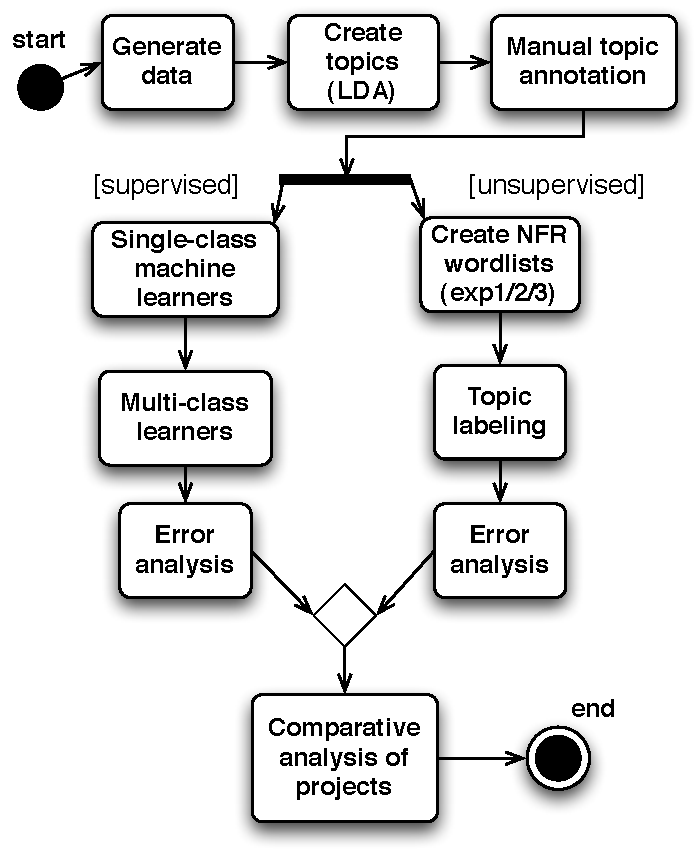
\includegraphics[width=.45\textwidth]{figures/process-model}
 \caption{Research methodology process view.}
  \label{fig:process}
\end{figure}

\subsection{Generating the data}
\label{sec:wordlist}
To evaluate our approach, we sought candidate systems that were mature projects and had openly accessible source control repositories. We selected systems from the same application domain, so the functional requirements would be broadly similar. We selected MySQL and MaxDB as they were open-source, partially-commercial database systems. MaxDB started in the late 1970s as a research project, and was later acquired by SAP. As of version 7.500, released April 2007, the project has 940 thousand lines of C source code~\footnote{generated using David A. Wheeler's \emph{SLOCCount}.}. The MySQL project started in 1994 and MySQL 3.23 was released in early 2001. MySQL contains 320 thousand lines of C and C++ source code.  Choosing an older version of these projects allows us to focus on projects which have moved into the maintenance phase of the software life-cycle.

For each project, we used source control commit comments, the messages that programmers write when they commit revisions to a source control repository. This is the most readily accessible source of project interactions for outside researchers; bug reports and email messages were not available for both projects. An example of a typical commit message is: \textit{``history annotate diffs bug fixed (if mysql\-\_real\-\_connect() failed there were two pointers to malloc'ed strings, with memory corruption on free(), of course)''}. We extracted these messages and indexed them by creation time. We summarized each message as a word distribution but removed stop-words such as \emph{the} and \emph{at}. Stemming was performed in the later stages of our analysis.

From that data-set, we created an XML file which separated commits into 30 day periods. This size of period is smaller than the time between minor releases but large enough for there to be sufficient commits to analyze. For this set of periods, we created `topics' using Latent Dirichlet Allocation, a topic identification algorithm. 

Typically a topic analysis tool like LDA will try to find $N$ independent word distributions within the word distributions of all the messages. Linear combinations of these $N$ word distributions are then meant to be able to recreate the word distributions of all of the underlying messages. These $N$ word distributions effectively form topics: cross-cutting collections of words relevant to one or more of our commit messages. LDA extracts topics in an unsupervised manner; the algorithm relies solely on the source data with no human intervention.

In topic analysis a single document, such as a commit message, can be related to multiple topics. Representing documents as a mixture of topics maps well to source code repository commits, which often have more than one purpose~\cite{Hindle09ICSM}.  A topic represents both a word distribution and a group of commit log comments that are related to each other by their content.  In this paper a topic is a set of tokens extracted from commit messages found within a project's source control system (SCS).
\todo[inline]{These paragraphs should've come way earlier, in previous we should explain LDA so this doesn't need to be here.}

We applied Blei's LDA implementation~\cite{Blei2003} against the word distributions of these commits, and generated lists of topics per period. 
We set the number of topics to generate to $20$, because past experimentation, e.g. \cite{Hindle09ICSM}, showed that fewer topics might aggregate multiple unique topics while any more topics seemed to dilute the results and create indistinct topics. Furthermore, more than $20$ topics quickly became infeasible for inspection.

\subsection{Generating word lists}
Topics are word distributions: lists of words ranked by frequency, which can be burdensome to interpret and hard to distinguish and understand. While the topic models themselves are generated automatically, what to make of them is less clear. For example, in our previous work~\cite{Hindle09ICSM}, as well as in Baldi et al.~\cite{Baldi2008}, topics are named manually: human experts read the highest-frequency members of a topic and assign a keyword accordingly. E.g., for the word list \emph{``listener change remove add fire''}, Baldi et al. assign the keyword \emph{event-handling}. The labels are reasonable enough, but still require an expert in the field to determine them. We sought to automate the process of naming the topics.

Accordingly, we tried to associate each topic with a label from a list of keywords and related terms. We performed simple string matching between these topics and our lists, `naming' a topic if it contained that word or words (a topic might match several keywords). We used several different word lists for comparison, which we call \textsf{exp1, exp2, exp3} in the text which follows. 

Our first word list set, \textsf{exp1}, was generated using the ontology described in Kayed et al.~\cite{5072519}. That paper constructs an ontology for software quality measurement using eighty source documents, including research papers and international standards. The labels we used:
\begin{quotation}
\small \noindent \textsf{
integrity, security,
interoperability, testability, maintainability, traceability,
accuracy, modifiability, understandability, availability, modularity,
usability, correctness, performance, verifiability, efficiency,
portability, flexibility, reliability.
}
\end{quotation}

Our second word list set, \textsf{exp2}, relied on the ISO quality model (ISO9126)~\cite{iso9126}. ISO9126 describes six high-level non-functional requirements (listed in Table \ref{tbl:wnsig}). There is some debate about the significance and importance of the terms in this model. However, ISO9126 is ``an international standard and thus provides an internationally accepted terminology for software quality \cite[p. 58]{Boegh2008},'' that is sufficient for the purposes of this research. The terms extracted from ISO9126 may not capture all words associated with the labels.  For example, the term ``redundancy'' is one most would agree is relevant to discussion of reliability, but is not in the standard. We therefore took the words from the taxonomy and expanded them.

To construct these expanded word lists, we used WordNet~\cite{Fellbaum1998}, an English-language ``lexical database'' that contains semantic relations between words, including common related forms (similar to word stemming), meronymy and synonymy. We then added Boehm's 1976 software quality model \cite{Boehm+:1976:ICSE}, and classified his eleven `ilities' into their respective ISO9126 qualities. We did the same for the quality model produced by McCall et al. \cite{mccall1977}. Finally, we analyzed two mailing lists from another software project to expand our set with domain-specific terms. For example, we add the term ``performance'' to the synonyms for \emph{efficiency}, since this term occurs in most mail messages that discuss efficiency.

For the third list of quality labels,  \textsf{exp3}, we extended the list from \textsf{exp2} using unfiltered WordNet similarity matches. Similarity in WordNet means siblings in a hypernym tree. We do not include these words here for space considerations (but see the Appendix for our data repository). It is not clear the words associated with our labels are specific enough, however: for example, the label \emph{maintainability} is associated with words \emph{ease} and \emph{ownership}.

\begin{table*}
	\centering
\begin{tabular}{c|p{9cm}}
\toprule
\textbf{Label} & \textbf{Related terms} \\
\midrule
\emph{Maintainability} &
testability changeability analyzability stability maintain maintainable modularity modifiability understandability interdependent dependency encapsulation decentralized modular\\ \hline
\emph{Functionality} &
security compliance accuracy interoperability suitability functional practicality functionality compliant exploit certificate secured ``buffer overflow'' policy malicious trustworthy vulnerable vulnerability accurate secure vulnerability correctness accuracy\\ \hline
\emph{Portability} &
conformance adaptability replaceability installability portable movableness movability portability specification migration standardized l10n localization i18n internationalization documentation interoperability transferability\\ \hline
\emph{Efficiency} &
``resource behaviour'' ``time behaviour'' efficient efficiency performance profiled optimize sluggish factor penalty slower faster slow fast optimization\\ \hline
\emph{Usability} &
operability understandability learnability useable usable serviceable usefulness utility useableness usableness serviceableness serviceability usability gui accessibility menu configure convention standard feature focus ui mouse icons ugly dialog guidelines click default human convention friendly user screen interface flexibility\\ \hline
\emph{Reliability} &
``fault tolerance'' recoverability maturity reliable dependable responsibleness responsibility reliableness reliability dependableness dependability resilience integrity stability stable crash bug fails redundancy error failure\\ 
\bottomrule
\end{tabular}
	\caption{NFRs and associated signifiers -- \textsf{exp2}}
	\label{tbl:wnsig}

\end{table*}

\todo[inline]{There should be a section here which is about manual annotation. It is really important and it is required by both analyses. Plus we can tell them how.}


\subsection{Unsupervised labelling}
% word list similarity
Using our three word lists, we labeled our topics where there was a match between the list and the topic. In general, this approach did not work out well as common labels dominated the less common labels. The related words for \emph{correctness}, for example, tended to be too lengthy and non-specific. 
Table \ref{tbl:wordlist} lists broad labeling results for MaxDB as an example. A \emph{named topic} is a topic with a matching label. There are \{periods X 20\} topics per project as we told LDA to extract 20 topics per period. All experiments were run on MaxDB 7.500 and MySQL 3.23 data.

%\todo[inline,color=green]{this table should have mysql}
\begin{table}

% % This data came from running  
% %   python check_validity.py
% %  in src/validate
% % and then running
% % tail -n 5 *maxdb*yes_no*
% % tail -n 5 *mysql*yes_no*
% ok the new way is to run lda_relator
% src/validate/lda_relator_counts.sh
	\centering
\begin{tabular}{l|c|c|c|c}
\toprule
Project & Measure & \textsf{exp1} & \textsf{exp2} & \textsf{exp3} \\
\midrule
% NOTE THESE WERE THE OLD VALUES
% WHY DID THEY CHANGE???
% DUNNO
%Named topics   & 281 & 125 & 328  \\
%Unnamed topics & 139 & 295 & 92   \\

% these were check_validate
% MaxDB 7.500 & Named Topics   & 305 & 183 & 330 \\
% MaxDB 7.500 & Unnamed Topics & 84  & 206 & 59   \\
% MaxDB 7.500 & Total  Topics  & 389 & 389 & 389 \\
% MySQL 3.23  & Named Topics   & 341 & 202 & 469 \\
% MySQL 3.23  & Unnamed Topics & 245 & 384 & 117 \\
% MySQL 3.23  & Total  Topics  & 586 & 586 & 586 \\

% these are lda relator

MaxDB 7.500 & Named Topics   & 281 & 125 & 328 \\ % these numbers are
                                % slightly different solely because
                                % we're counting empty topics
                                % maxdb has 80 empty topics
MaxDB 7.500 & Unnamed Topics & 219  & 375 &  172  \\
MaxDB 7.500 & Total  Topics  & 500 & 500 & 500 \\
MySQL 3.23  & Named Topics   & 524 & 273 & 773 \\
MySQL 3.23  & Unnamed Topics & 476 & 727 & 227 \\
MySQL 3.23  & Total  Topics  & 1000 & 1000 & 1000 \\


\bottomrule
\end{tabular}
	\caption{Automatic topic labelling for MaxDB 7.500}
	\label{tbl:wordlist}

\end{table}

For \textsf{exp1}, our best performing labels (the labels matched with the most topics) were \emph{correctness} (182 topics) and \emph{testability} (121). We did not get good results for usability or accuracy, which were associated with fewer than ten topics. We also looked for correlation between our labels: Excluding double matches (self-correlation), our highest co-occurring terms were verifiability and traceability, and testability and correctness (76 and 62 matches, respectively).

For \textsf{exp2}, there are many more unnamed topics. Only reliability produces a lot of matches, mostly with the word `error'. Co-occurrence results were poor.

For \textsf{exp3}, we had many more named topics. As we mentioned, the word-lists are quite broad, so there are likely to be false-positives. See the following sections for our error analysis. We found a high of 265 topics for usability, with a low of 44 topics for maintainability. Common co-occurrences were reliability and usability, efficiency and reliability, and efficiency and usability (200, 190, and 150 topics in common, respectively). 


\subsubsection{Analysis of the unsupervised labelling}

\label{sec:unsuplabelling}

Based on the labels, and our manual topic labelling, we compared the results of the unsupervised word matching approach. For each quality we tried to assess whether the manual tag matched the unsupervised label assigned. Figure \ref{fig:maxdb-unsup-results} shows our results for MaxDB and MySQL. Our error is measured using the ROC area-under-curve value. This value is the area under the Receiver Operating Characteristic (\emph{ROC}) curve, sometimes referred to as \emph{AUC}. ROC values reflect a score, similar to school letter-grades (A is 0.9, C is 0.6), reflecting how well a particular learner performed for the given data. A ROC result of 0.5 would be equivalent to a random learner (randomly classifying data). ROC maps to the more familiar concepts of precision/sensitivity and recall/specificity: it plots the true positive rate (sensitivity) versus the false positive rate (1 - specificity). A perfect learner has a ROC value of 1.0, reflecting perfect recall and precision.

\begin{figure*}
  \centering
 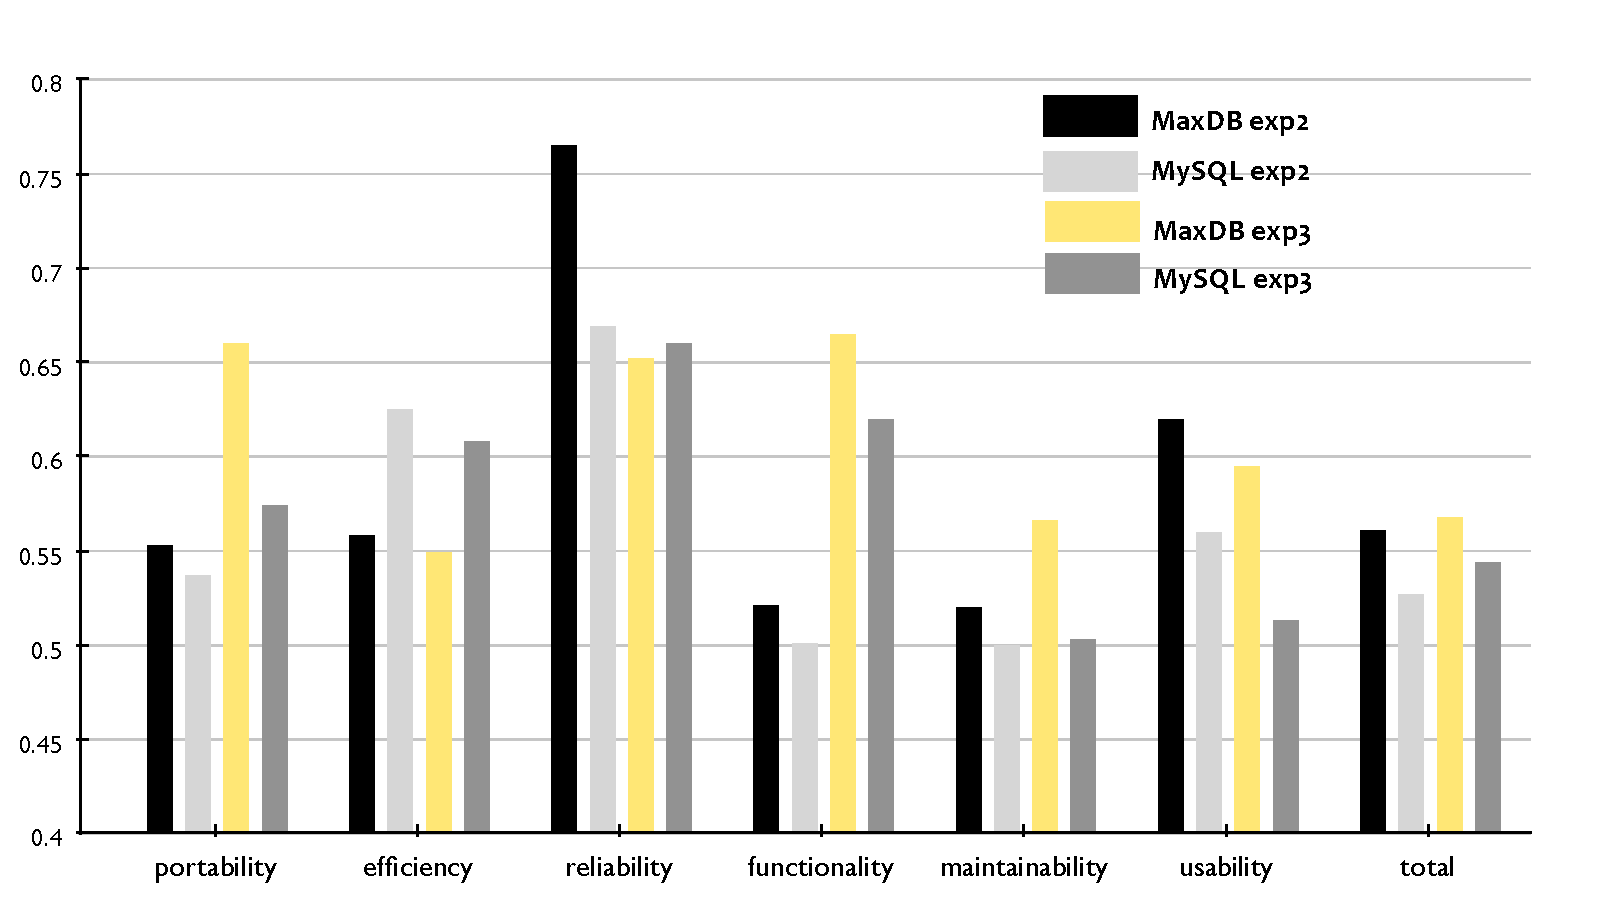
\includegraphics[width=.85\textwidth]{figures/unsupervised-bar}
 \caption{ROC values for each NFR, per project and wordlist.}
%\todo[inline]{this is too tiny in print}

  \label{fig:maxdb-unsup-results}
\end{figure*}


Based on these results we find that reliability and usability worked well for MaxDB in \textsf{exp2} and better in \textsf{exp3}. MySQL had reasonable results within \textsf{exp2} for reliability and efficiency. MySQL's results for efficiency did not improve in \textsf{exp3} but other qualities such as functionality did improve. If a \emph{C} grade performance has a ROC value of $0.6$ then most of these tests scored a grade of \emph{C} or less, but our results were still better than random chance.


\subsection{Supervised labelling}
\label{sec:suplearn}
Supervised labelling requires expert analysis of the correct word to assign to a topic. %In order to validate how effective these word-bag approaches to topic labelling would be we created a validation data set. 
 For MySQL 3.23 and MaxDB 7.500, we manually annotated each extracted topic in each period with the same NFR labels as \textsf{exp2} (software qualities). We looked at each period's topics, and assessed what the data -- consisting of the frequency-weighted word lists and messages -- suggested was the topic for that period. We were able to pinpoint the appropriate label using auxiliary information as well, such as the actual revisions and files that were related to this topic. For example, for the MaxDB topic consisting of a message ``exit() only used in non NPTL LINUX Versions'', we tagged that topic \emph{portability}. We compared against this data-set, but we also used it for our supervised learning based topic classification. A topic may have more than one matching keyword.
\todo[inline]{inter-rater reliability }

We used a suite of supervised classifiers from WEKA~\cite{weka09}. WEKA is a suite of machine learning tools such as support vector machines and Bayes nets. We also used the multi-labelling add-on for WEKA, Mulan~\cite{mulan}\footnote{\url{http://mlkd.csd.auth.gr/multilabel.html}}. Traditional classifiers map our topics to a single class, whereas Mulan allows for a mixture of classes per topic, which maps to what we observed while manually labelling topics.

To assess the performance of the supervised learners, we did a 10-fold cross-validation~\cite{Kohavi1995}, a common technique for evaluating machine learners. The original data is partitioned randomly into ten subsamples. One subsample is used as a training set and evaluated on the other nine subsamples. This is repeated nine more times, with each subsample used once as the training set. We have reported these results below in Section \ref{sec:suplabelling}.

\subsubsection{Analysis of the supervised labelling}
\label{sec:suplabelling}
Because our data-set was of word counts we expected Bayesian techniques, often used in spam filtering, to perform well. We tried other learners that WEKA~\cite{weka09} provides: rule learners, decision tree learners, vector space learners, and support vector machines.  Figure \ref{fig:best-learn-per-tag} shows the performance of the best performing learner per label.  We considered the best learner for a label to be the one which had the highest ROC value for that label. Figure \ref{fig:best-learn-per-tag} uses the ZeroR learner as a baseline, a common practice in machine learning. ZeroR naively chooses the largest category all of the time. It occasionally outperforms non-naive learners; for labels which are not as common, this is to be expected because any miscategorization will hurt accuracy. This is why we use ROC values, as they can better represent performance on labels which are not applicable to the majority of samples.

Figure \ref{fig:best-learn-per-tag} shows that MaxDB and MySQL have quite different results, as the ROC values for reliability and functionality seem swapped between projects. For both projects Bayesian techniques did the best out of a wide variety of machine learners tested. Discriminative Multinomial Naive Bayes (DMNBtext), Naive Bayes (NaiveBayes) and Multinomial Naive Bayes (NaiveBayesMultinomal) are all based on Bayes's theorem and all assume, naively, that the features are independent. The features we used are word counts per message. One beneficial aspect of this result is that it suggests we can have very fast training and classifying  since Naive Bayes can be calculated in $O(N)$ for $N$ features.
%http://nlp.stanford.edu/IR-book/html/htmledition/naive-bayes-text-classification-1.html

The less-frequently occurring a label the harder it is to get accurate
results, due to the high noise level. Nevertheless, these results are
better than our previous word bag results of \textsf{exp2} and
\textsf{exp3}, because the ROC values are sufficiently higher in most
cases (other than MaxDB reliability and MySQL efficiency). The
limitation of the approach we took here is that we assume labels are
independent; however, labels could be correlated with each other. 
The next section, Section \ref{sec:multilabel} on multi-labels
addresses the issue of a lack of independence and correlation between labels.
In the next section we will evaluate how well these learners perform
together.
%\todo[inline]{Comment about correlation, we should link to the Mulan section, perfect segway since Mulan relies on correlation.}



\begin{figure*}[ht]
\centering
\subfigure[MySQL]{
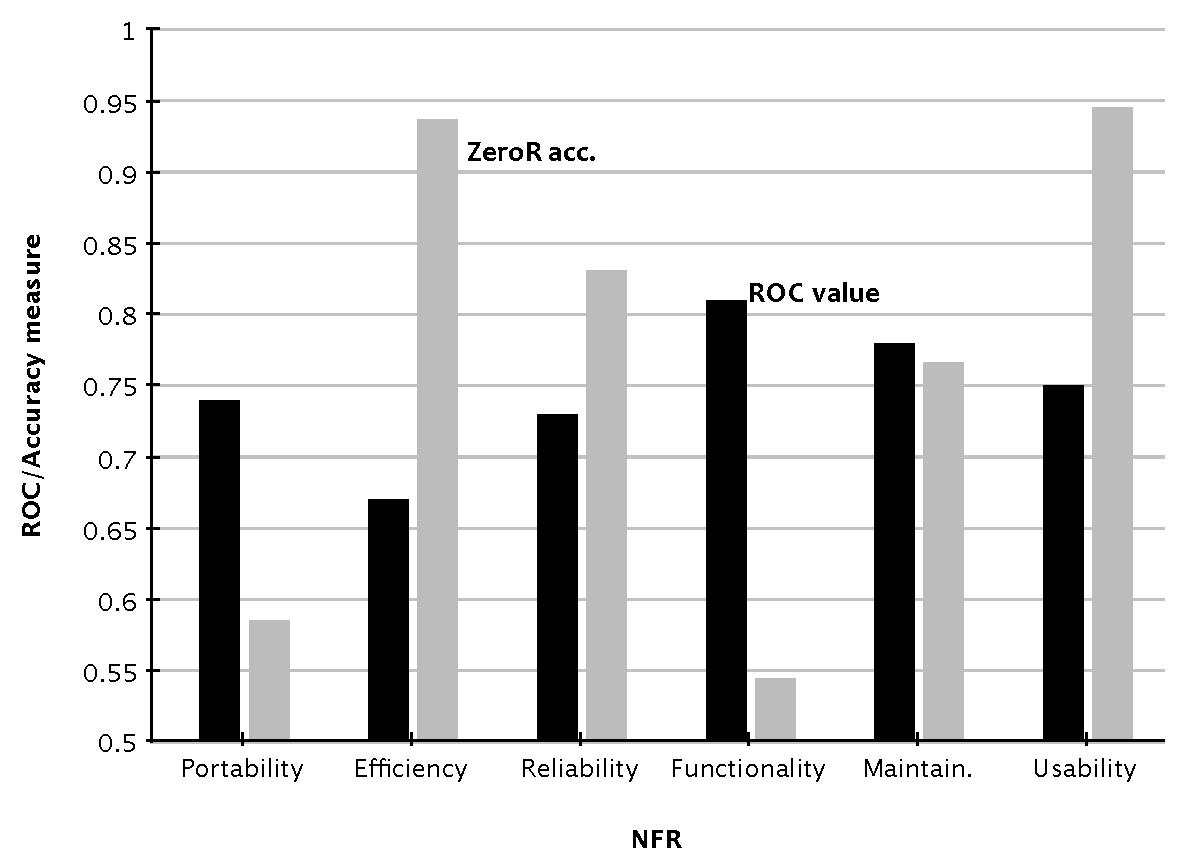
\includegraphics[width=0.4\textwidth]{figures/mysql-supervised}
\label{fig:subfig1}
}
\subfigure[MaxDB]{
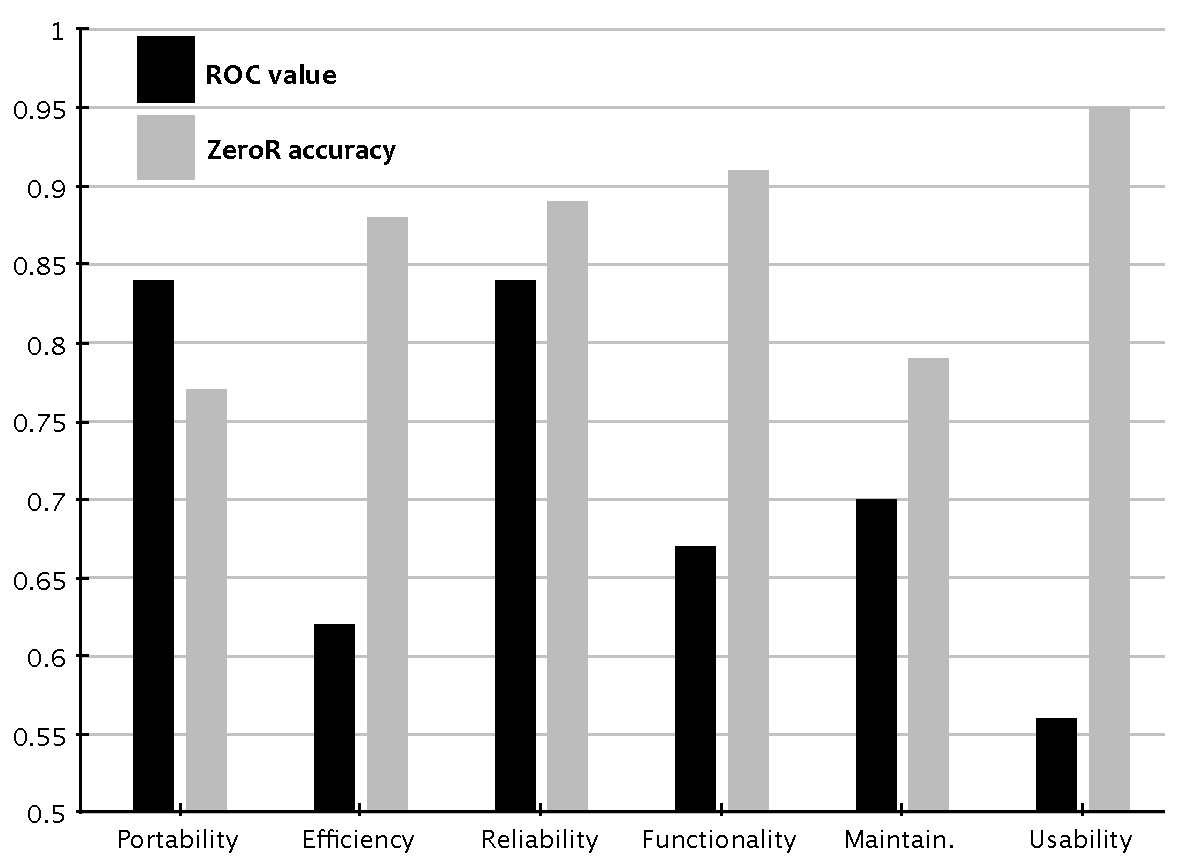
\includegraphics[width=0.4\textwidth]{figures/maxdb-supervised}
\label{fig:subfig2}
}
\label{fig:best-learn-per-tag}
\caption[]{ROC value for the best learner per label, compared with ZeroR accuracy values.  Possible values range from 0--1.
\todo[inline]{better discussion}
}
\end{figure*}

\subsection{Applying multiple labels to topics}
\label{sec:multilabel}

As noted in Section \ref{sec:wordlist}, each topic in our data-set can be composed of zero to all NFRs. For example, a commit message might address \textit{reliability} in the context of \textit{efficiency}, or make a \textit{maintainability} improvement in the source code that related to \textit{usability}. However, traditional machine learning techniques, such as Bayesian networks, can only map topics to a single class. The Mulan~\cite{mulan} library encapsulates several different machine learners which can handle this multi-label learning for our data-set. Mulan also includes methods for determining the performance of such techniques.
% TOO DETAILED The problem framed in the learners above has changed; instead of looking at the precision and recall of applying one label, we rank multiple labels at once. We must check if the full subset of labels was applied, and then how much of that subset was applied.

In multi-label learning the technique can perform micro or macro measurements. Macro measurements are aggregated at a class or label level. Micro measurements are aggregated at a decision level. So a macro-ROC measurement is the average ROC over the ROC values for all labels, where a micro-ROC is the average ROC over all examples that were classified. Unfortunately for MaxDB, the macro-ROC values are undefined because of poor performance of one of the labels.

Fig. \ref{fig:mulan} presents the results of Mulan's best multi-label
learners for our data. Calibrated Label Ranking (CLR) is a learner
that builds two layers, the first layer determines if an entity should
be labelled, while the second layer determines what labels should be assigned.
The Hierarchy Of Multi-label classifiERs (HOMER) and Binary Relevance (BR) act as a hierarchy of learners: BR is flat, while HOMER tries to build a deeper hierarchy to build a more accurate learner~\cite{mulan}. These classifiers performed better than other multi-label classifiers. They have the best micro and macro ROC scores, although their results are comparable to the naive Bayesian learners we used in Section \ref{sec:suplearn}.
\todo[inline]{discuss this similarity in more detail}
%\todo[inline]{what of CLR? Is it hierarchical?}

\begin{figure*}[ht]
\centering
\subfigure[MySQL]{
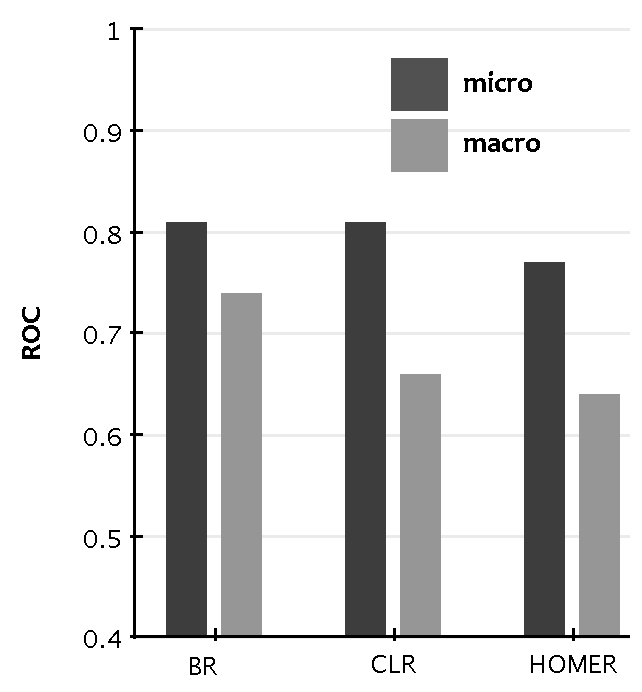
\includegraphics[width=0.4\textwidth]{figures/multi-label-results-mysql}
\label{fig:subfig3}
}
\subfigure[MaxDB]{
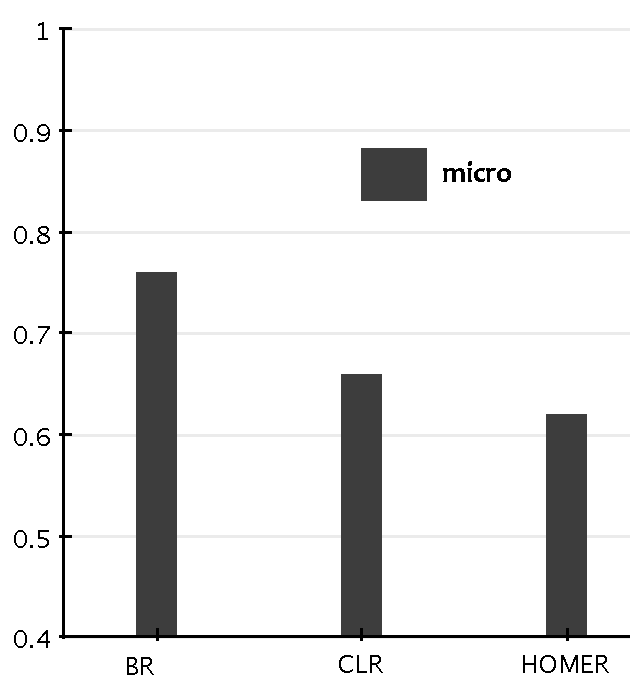
\includegraphics[width=0.4\textwidth]{figures/multi-label-results-maxdb}
\label{fig:subfig4}
}
\label{fig:mulan}
\caption[]{MySQL and MaxDB macro (grey) and micro (black) ROC results per multi-label learner. Possible values range from 0--1.
\todo[inline]{better discussion}% and graphical legend would be nice}
}
\end{figure*}

\subsection{Summary of techniques}
While unsupervised techniques (LSI and LDA are both unsupervised) are appealing in their lack of human intervention, and thus lower effort, supervised learners have the advantage of domain knowledge which typically means improved results.

Very rarely did \textsf{exp2} and \textsf{exp3} (naive word matching) ever perform as well as the supervised machine learners. For MaxDB, \textit{reliability} was slightly better detected using the static word list of \textsf{exp2}. In general, the machine learners and \textsf{exp3} did better than \textsf{exp2} for both MaxDB and MySQL. For both MySQL and MaxDB \textit{usability} was better served by \textsf{exp2}. \textit{Usability} was a very infrequent label, however, which made it difficult to detect in any case.

We found that the multi-label learners of BR, CLR and HOMER did not do as well for Macro-ROC as NaiveBayes and other NaiveBayes derived learners. This suggests that by sticking together multiple NaiveBayes learners we could probably label sets of topics effectively, but it would require a separate NaiveBayes learner per label.

\section{NFRs and evolution} 
\todo[inline]{talk about this topic in one section}
\todo[inline]{reference project name Nomen more}
Using the classification results from the previous sections, we evaluated two research questions:
\begin{enumerate}
\item Do label frequencies change over time? That is, is a certain quality of more interest at one point in the life-cycle than some other? 
\item  Do the different projects differ in their relative topic interest? That is, is a particular quality more important to one project than the other projects?  
\end{enumerate}


\subsection{Visualization}
We created two visualizations of the manually labelled data. A problem we faced while visualizing was how to display tag overlaps. Our solution, while not optimal, was to assign a separate colour to each distinct set of annotations. Figures \ref{fig:maxdb} and \ref{fig:mysql} show extracted topics grouped by annotations. Annotations or labels that occur in adjacent windows are joined together as trends. For MaxDB (Figure \ref{fig:maxdb}) the largest trends were related to maintainability and portability. MaxDB supports numerous platforms and portability was a constant issue facing the project's development. MySQL was different, with many topics overlapping, so there were many different subsets. Functionality trends were prevalent throughout its history (the largest reddish streak across the top). Two combination  tags of ``functionality portability'' (orange) and ``maintainability portability'' (teal) streaked across most of the history of MySQL. Since this was MySQL 3.23, a stable branch, we expect that issues dealing with portability and maintenance would be the primary concerns of this branch: developers probably wanted it to work with current systems and thus had to update it.

\todo[inline]{Update this}


\begin{figure*}
  \centering
  % hi-res version
  %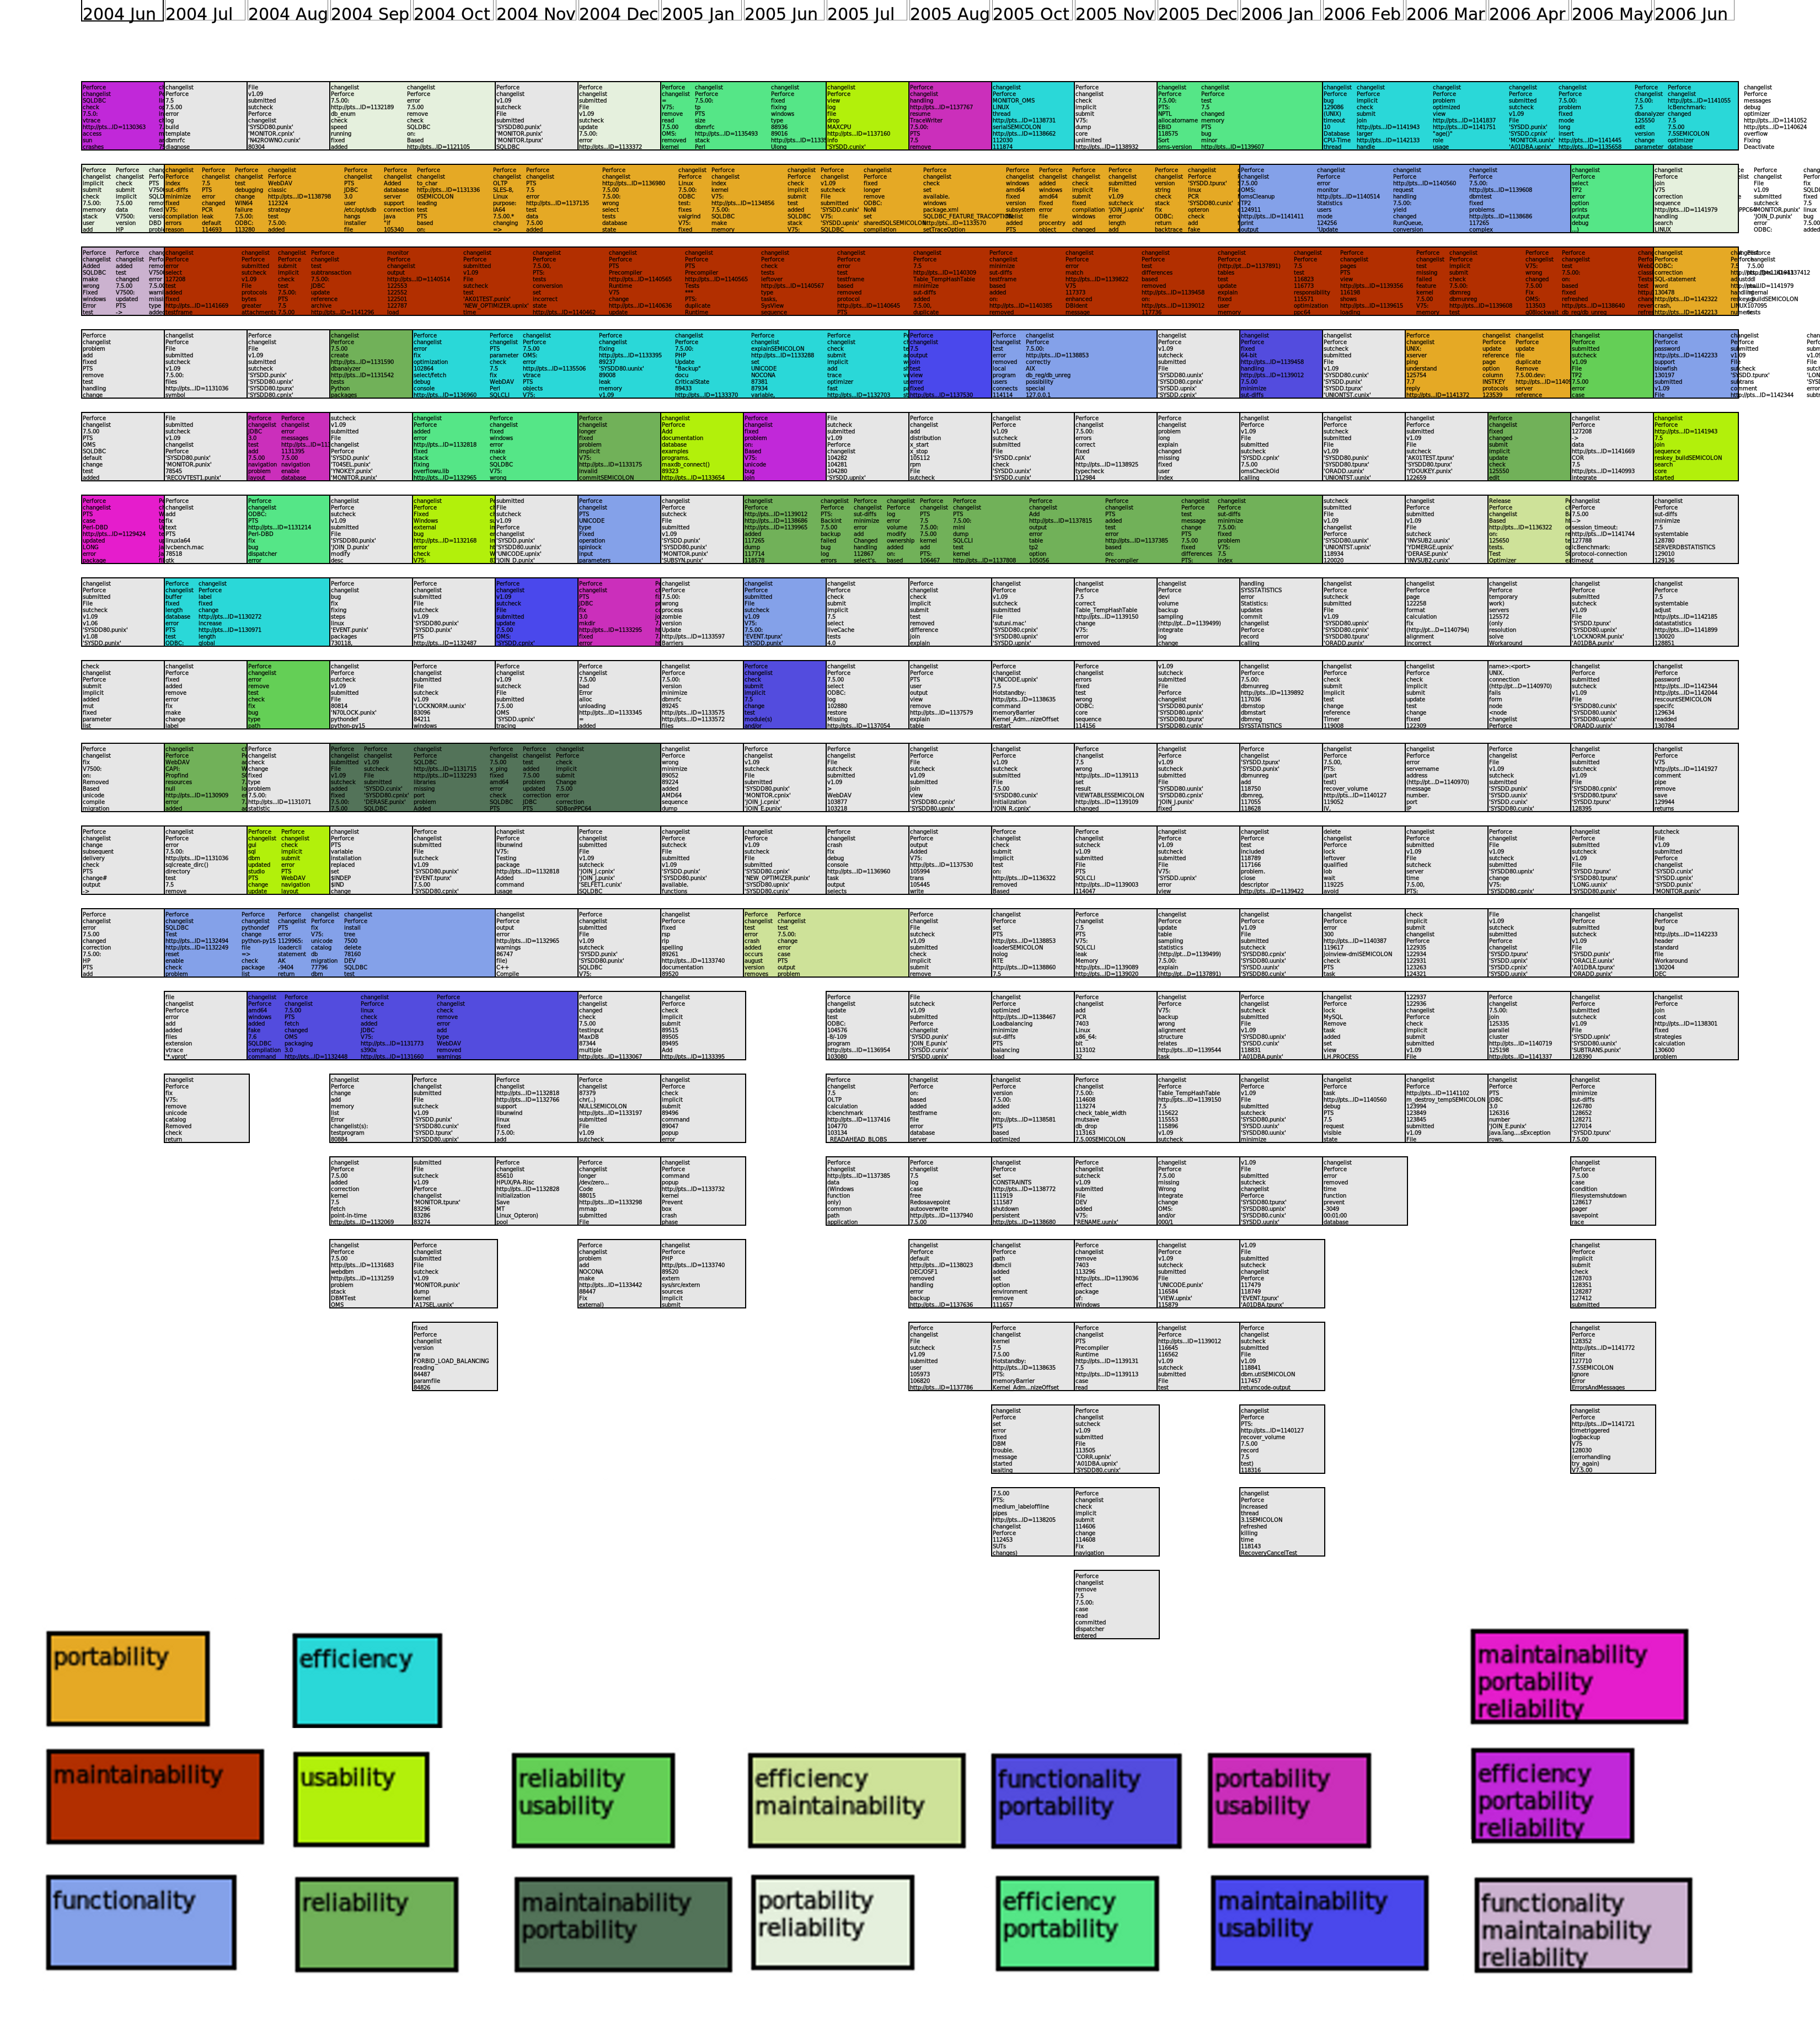
\includegraphics[height=.55\textheight]{maxdb-time-smear-plot-Equal}
  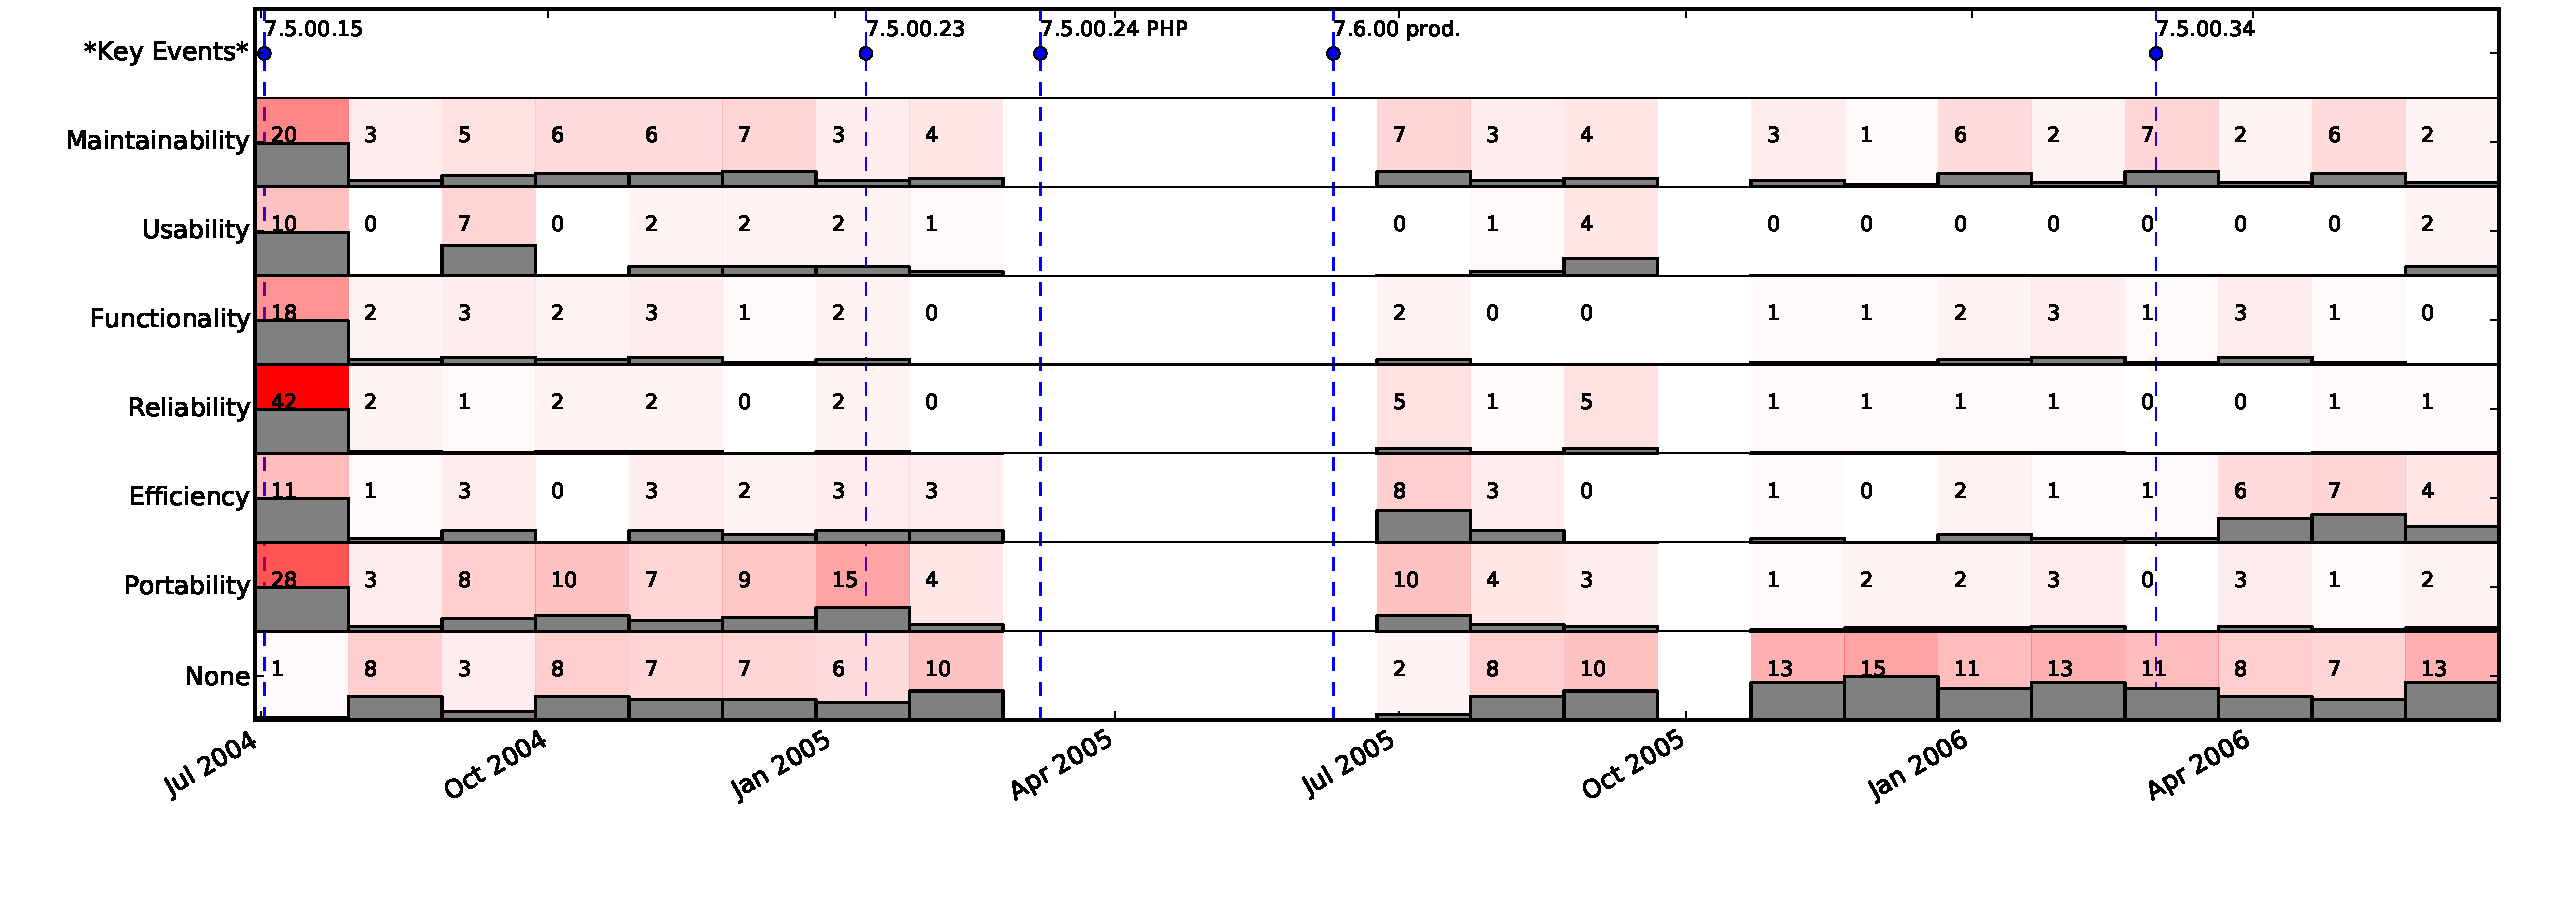
\includegraphics[width=\textwidth]{figures/maxdb-timeline}
  % 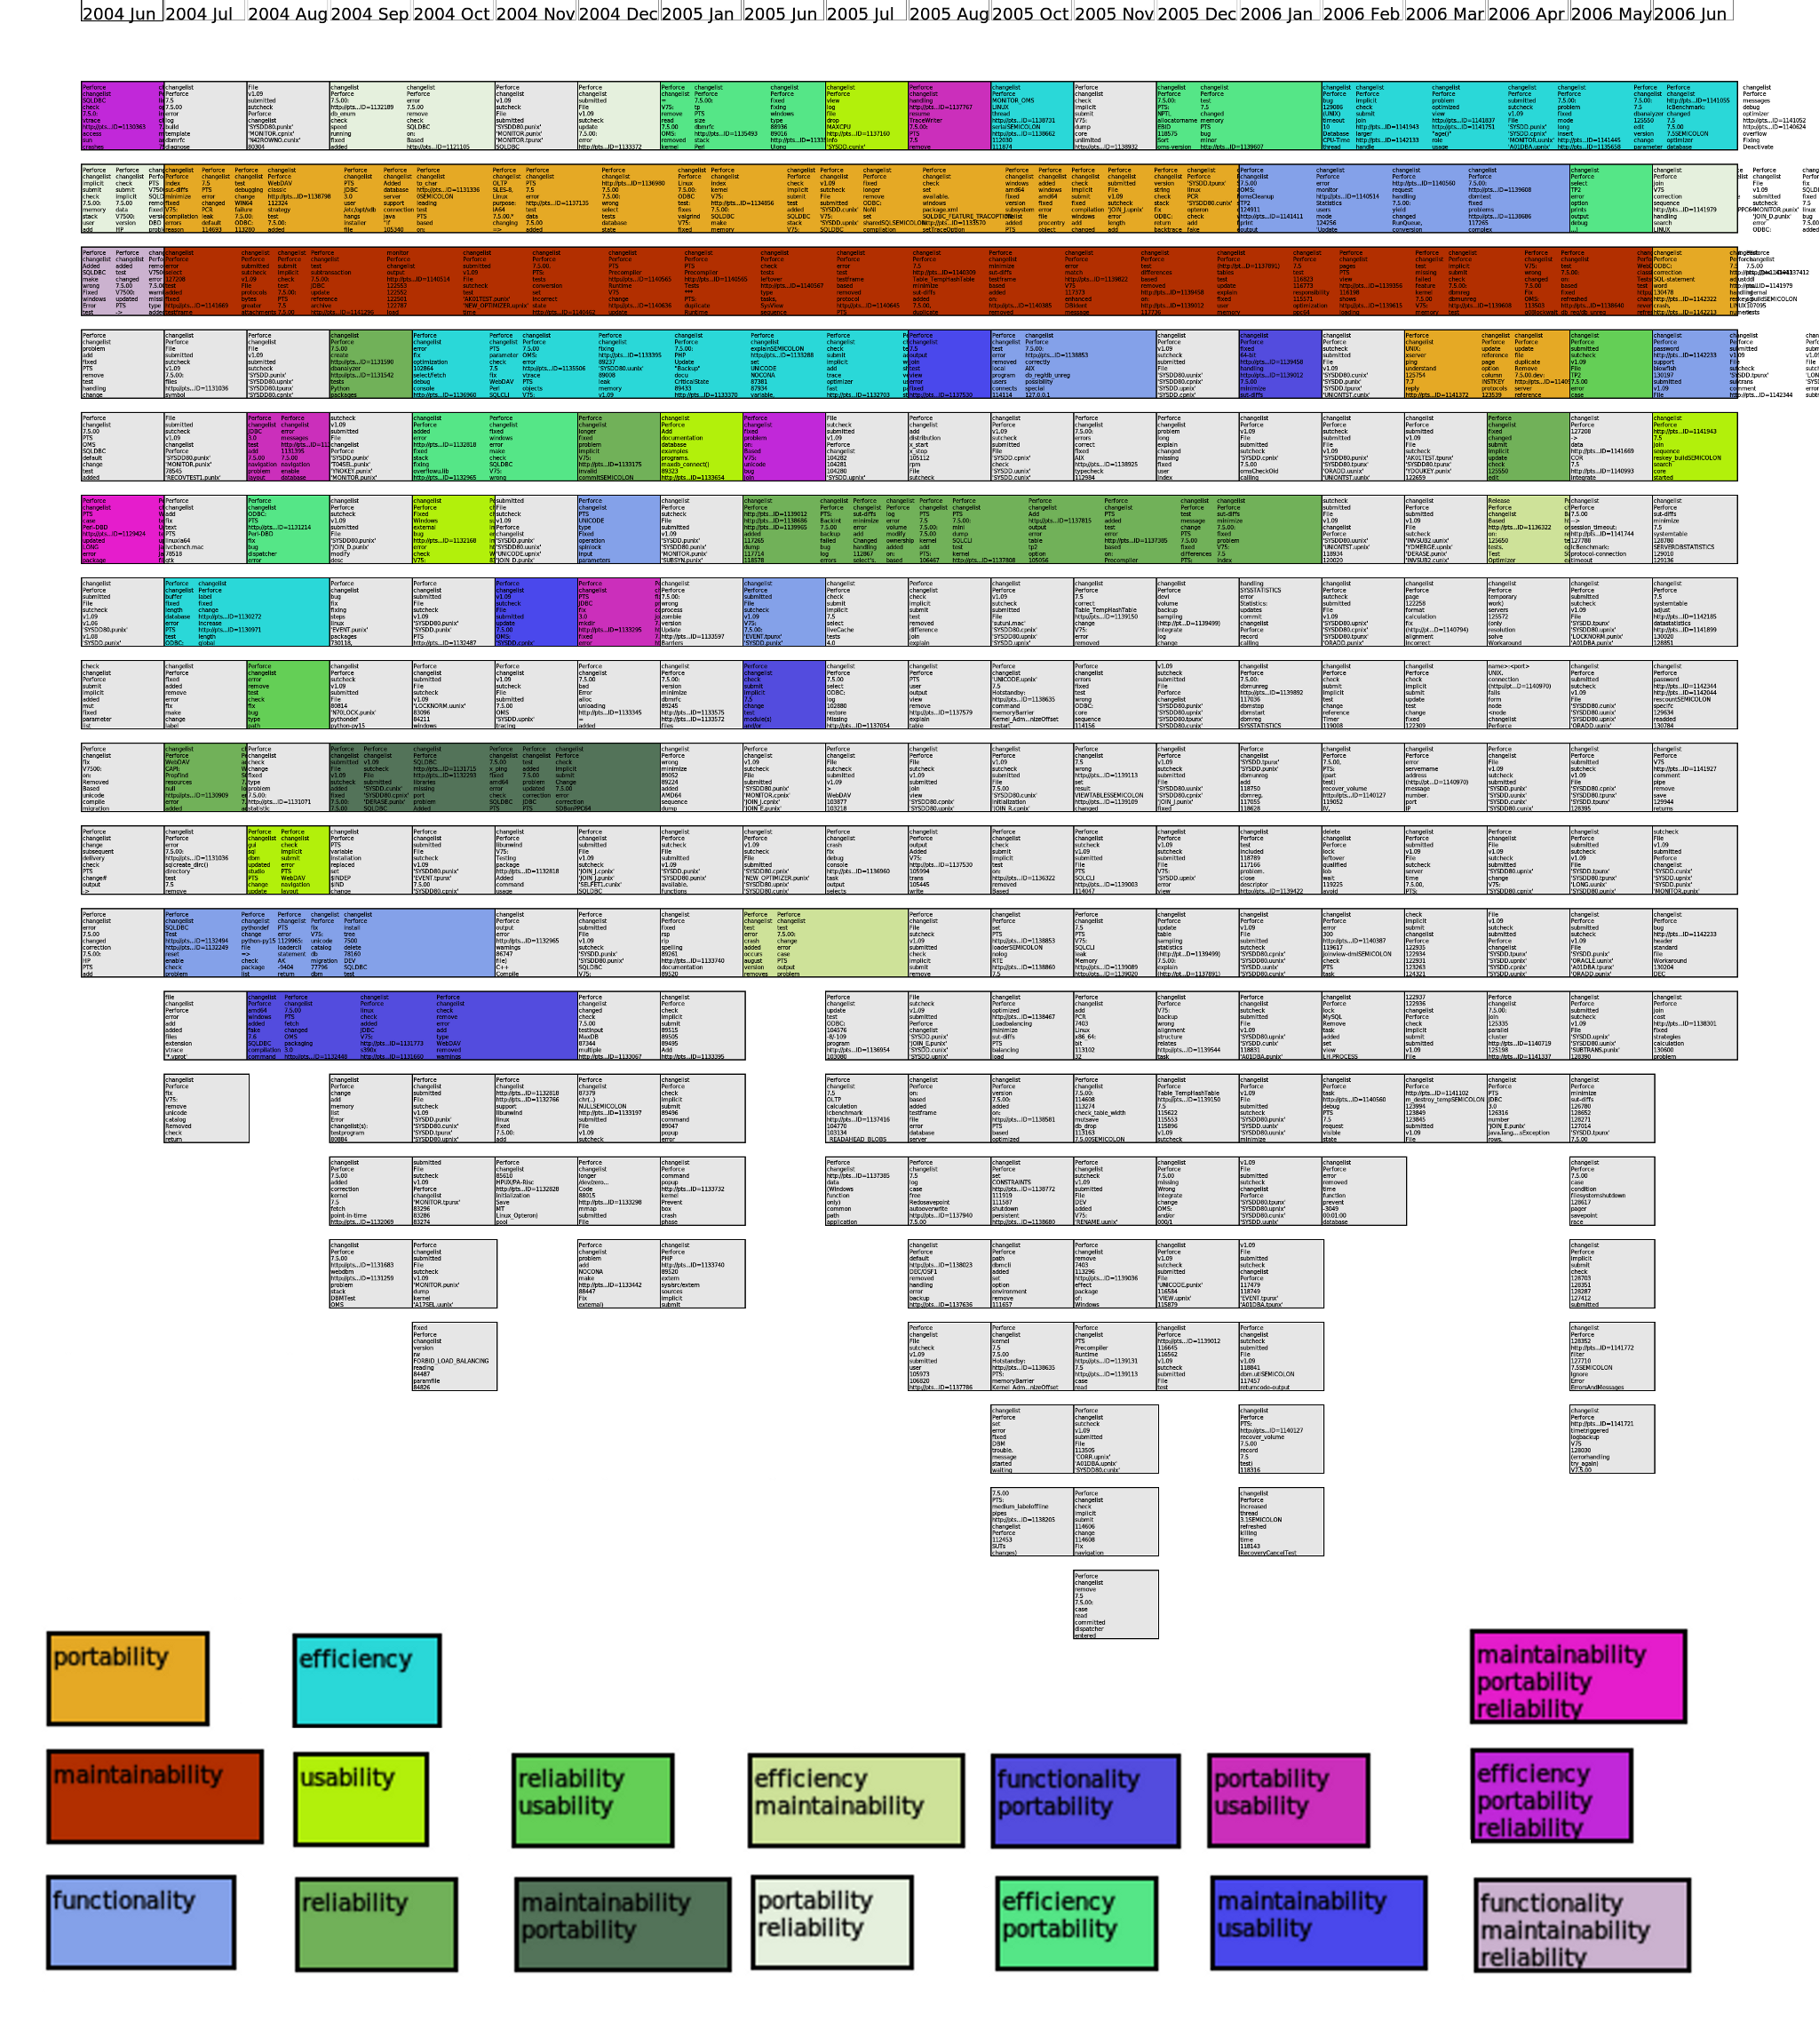
\includegraphics[height=.57\textheight]{small-maxdb-time-smear-plot-Equal}
 % \caption{MaxDB 7.500: Labelled topics related to non-functional software qualities plotted over time, continuous topics are trends that occur across time}
  \caption{MaxDB 7.500: NFRs over time. Topic frequency relative to that quality is mapped to alpha (transparency) value.}
 \label{fig:maxdb}
\end{figure*}

\begin{figure*}%[h]
  \centering
 %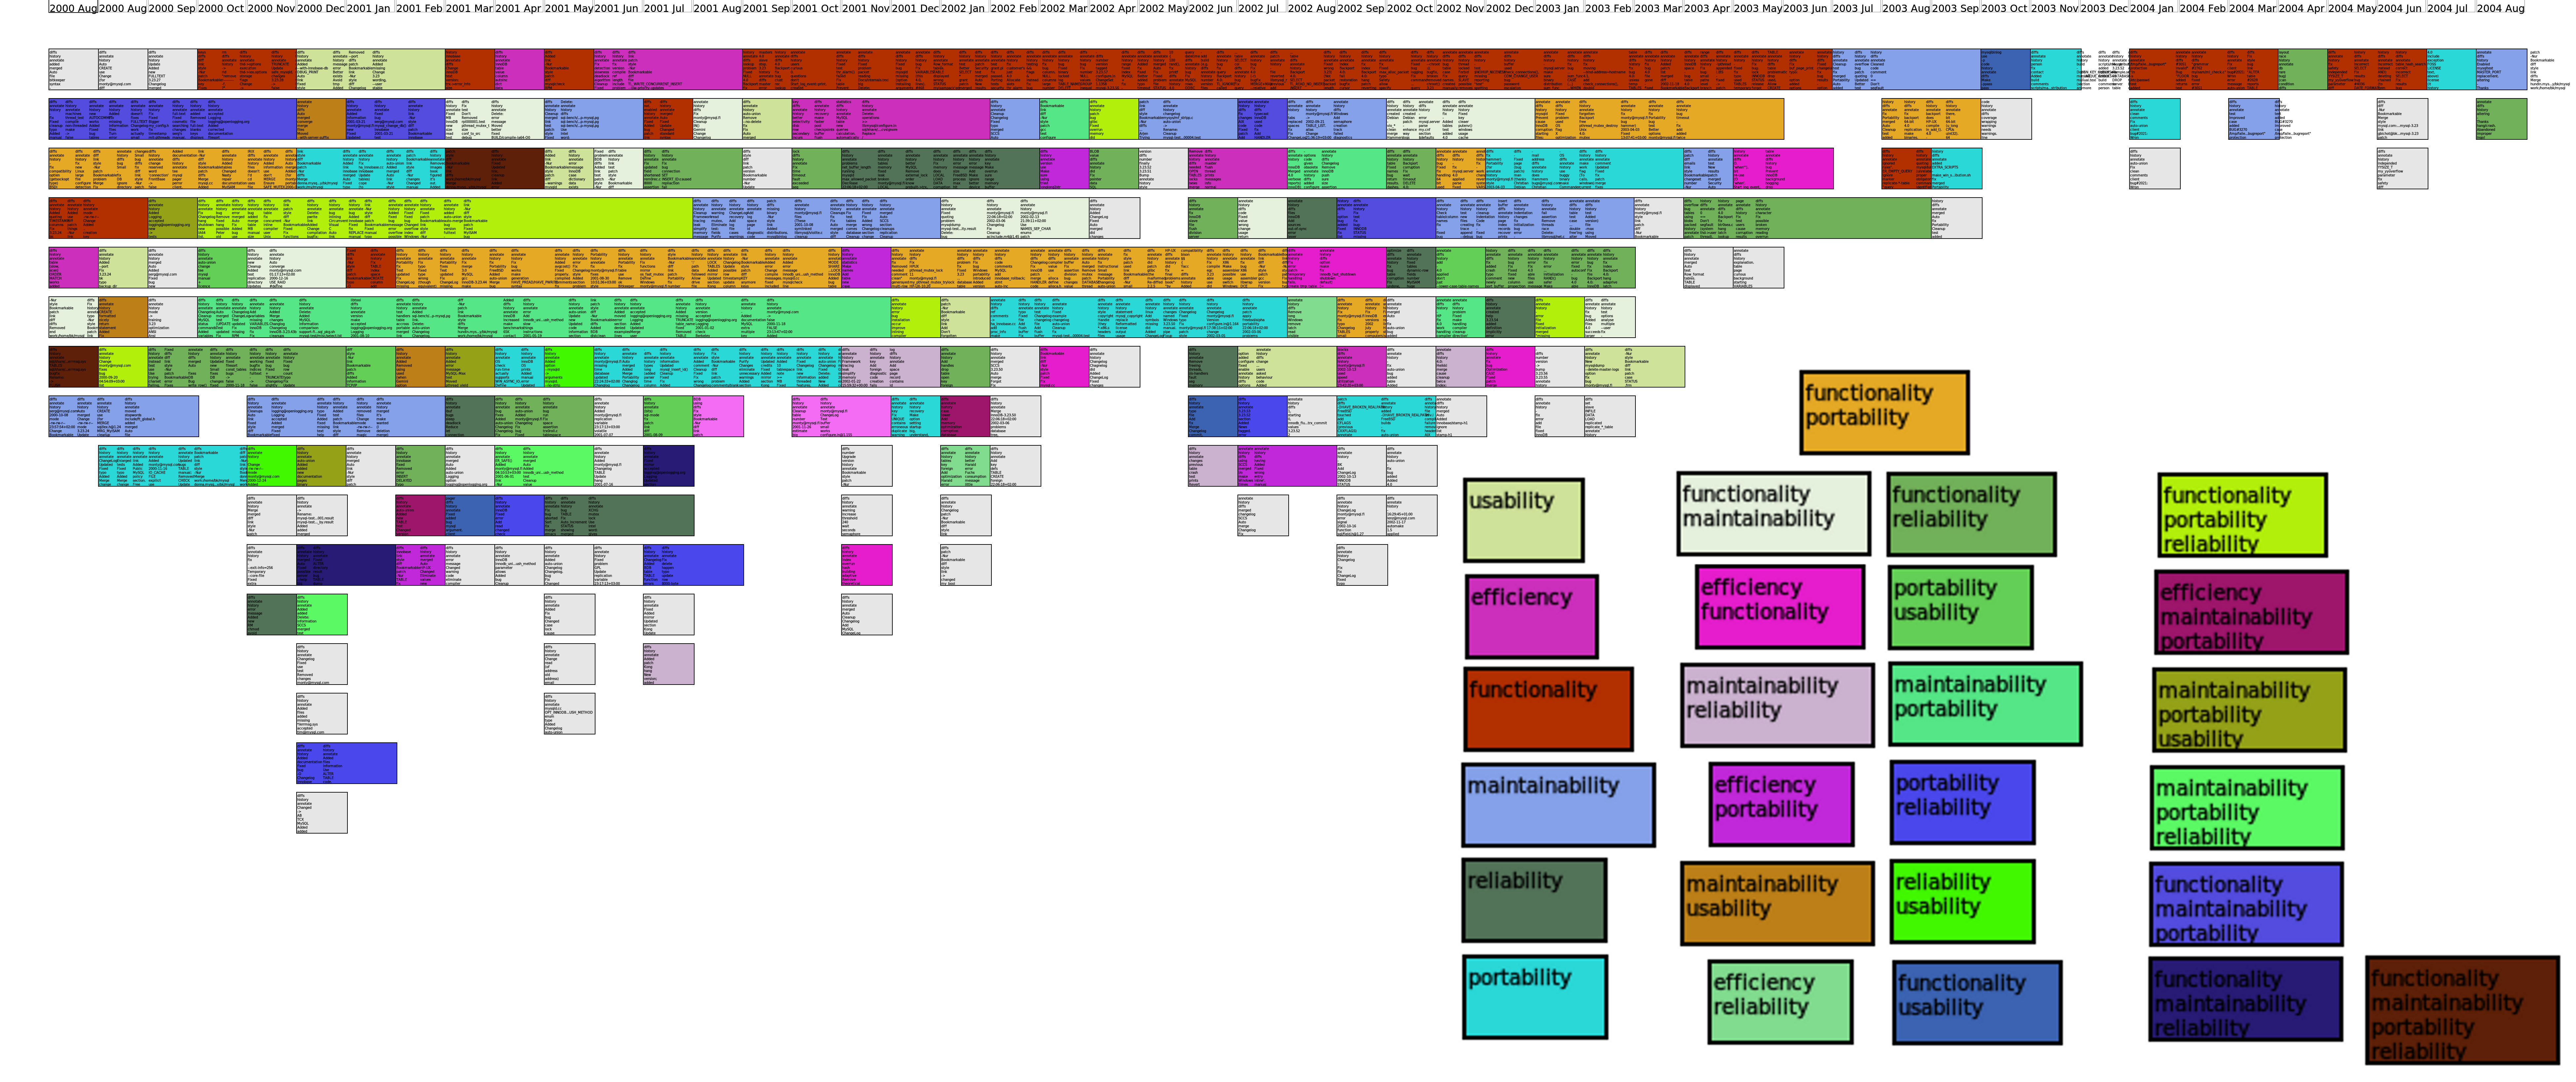
\includegraphics[width=.97\textwidth]{mysql-time-smear-plot-Equal}
  %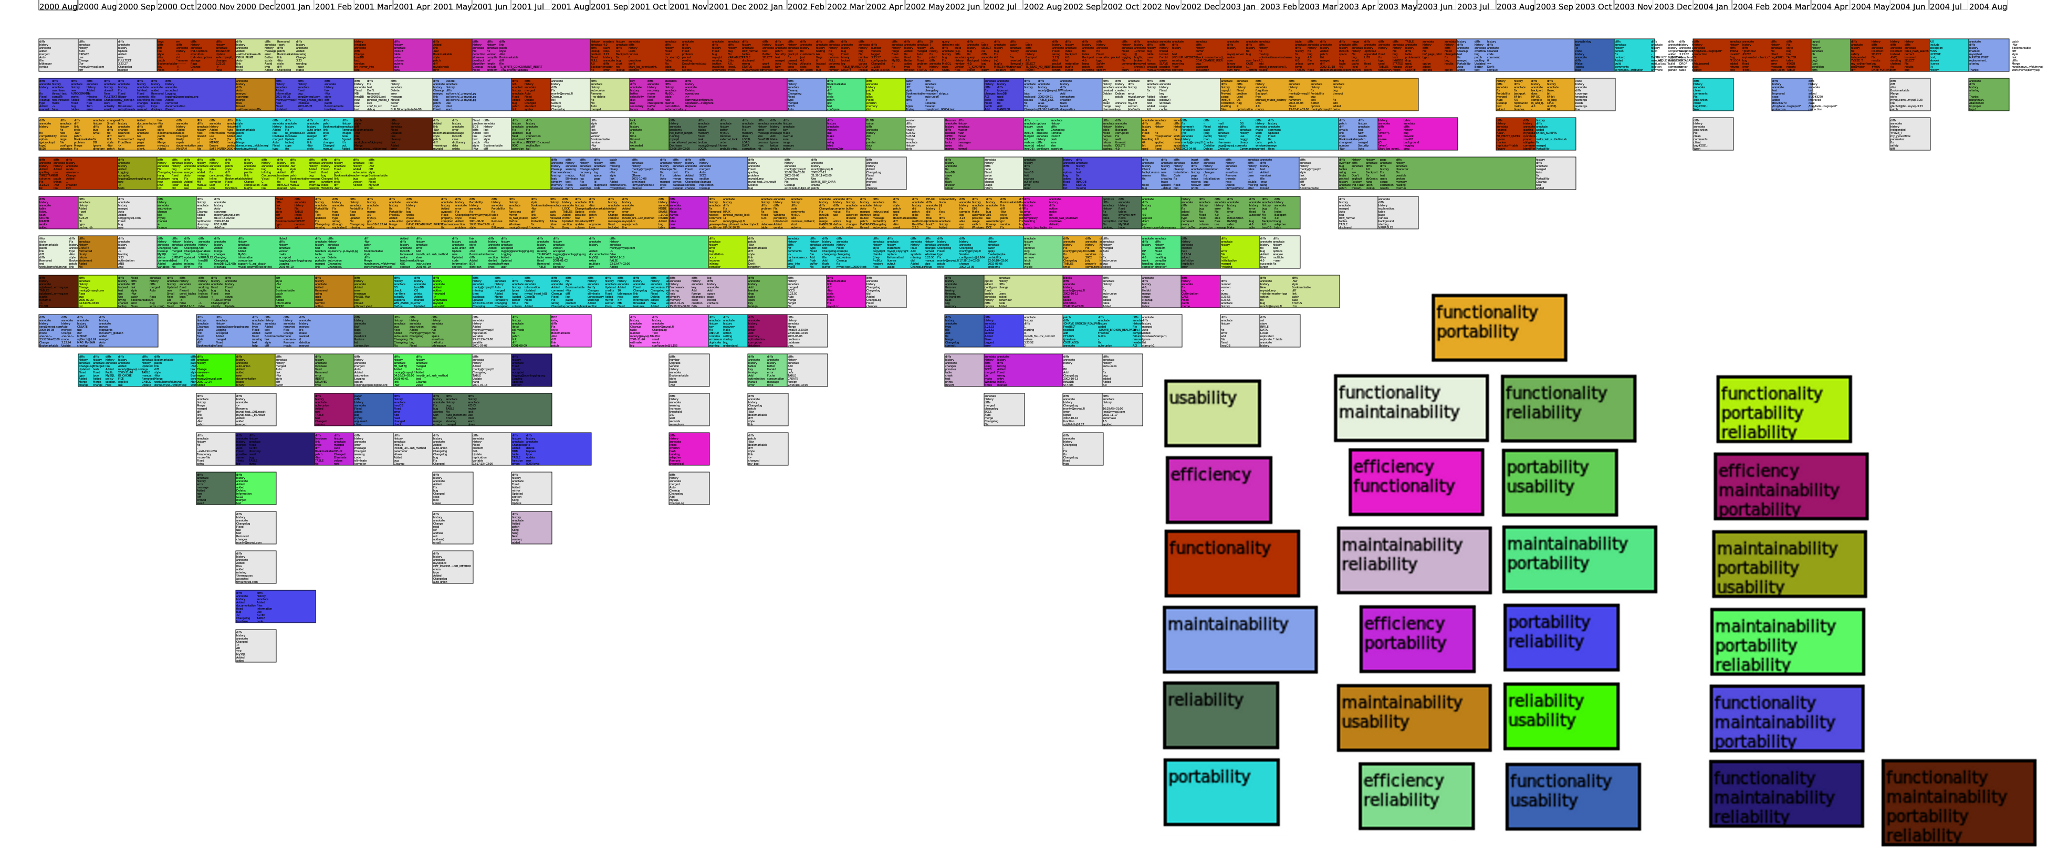
\includegraphics[width=.97\textwidth]{small-mysql-time-smear-plot-Equal}
  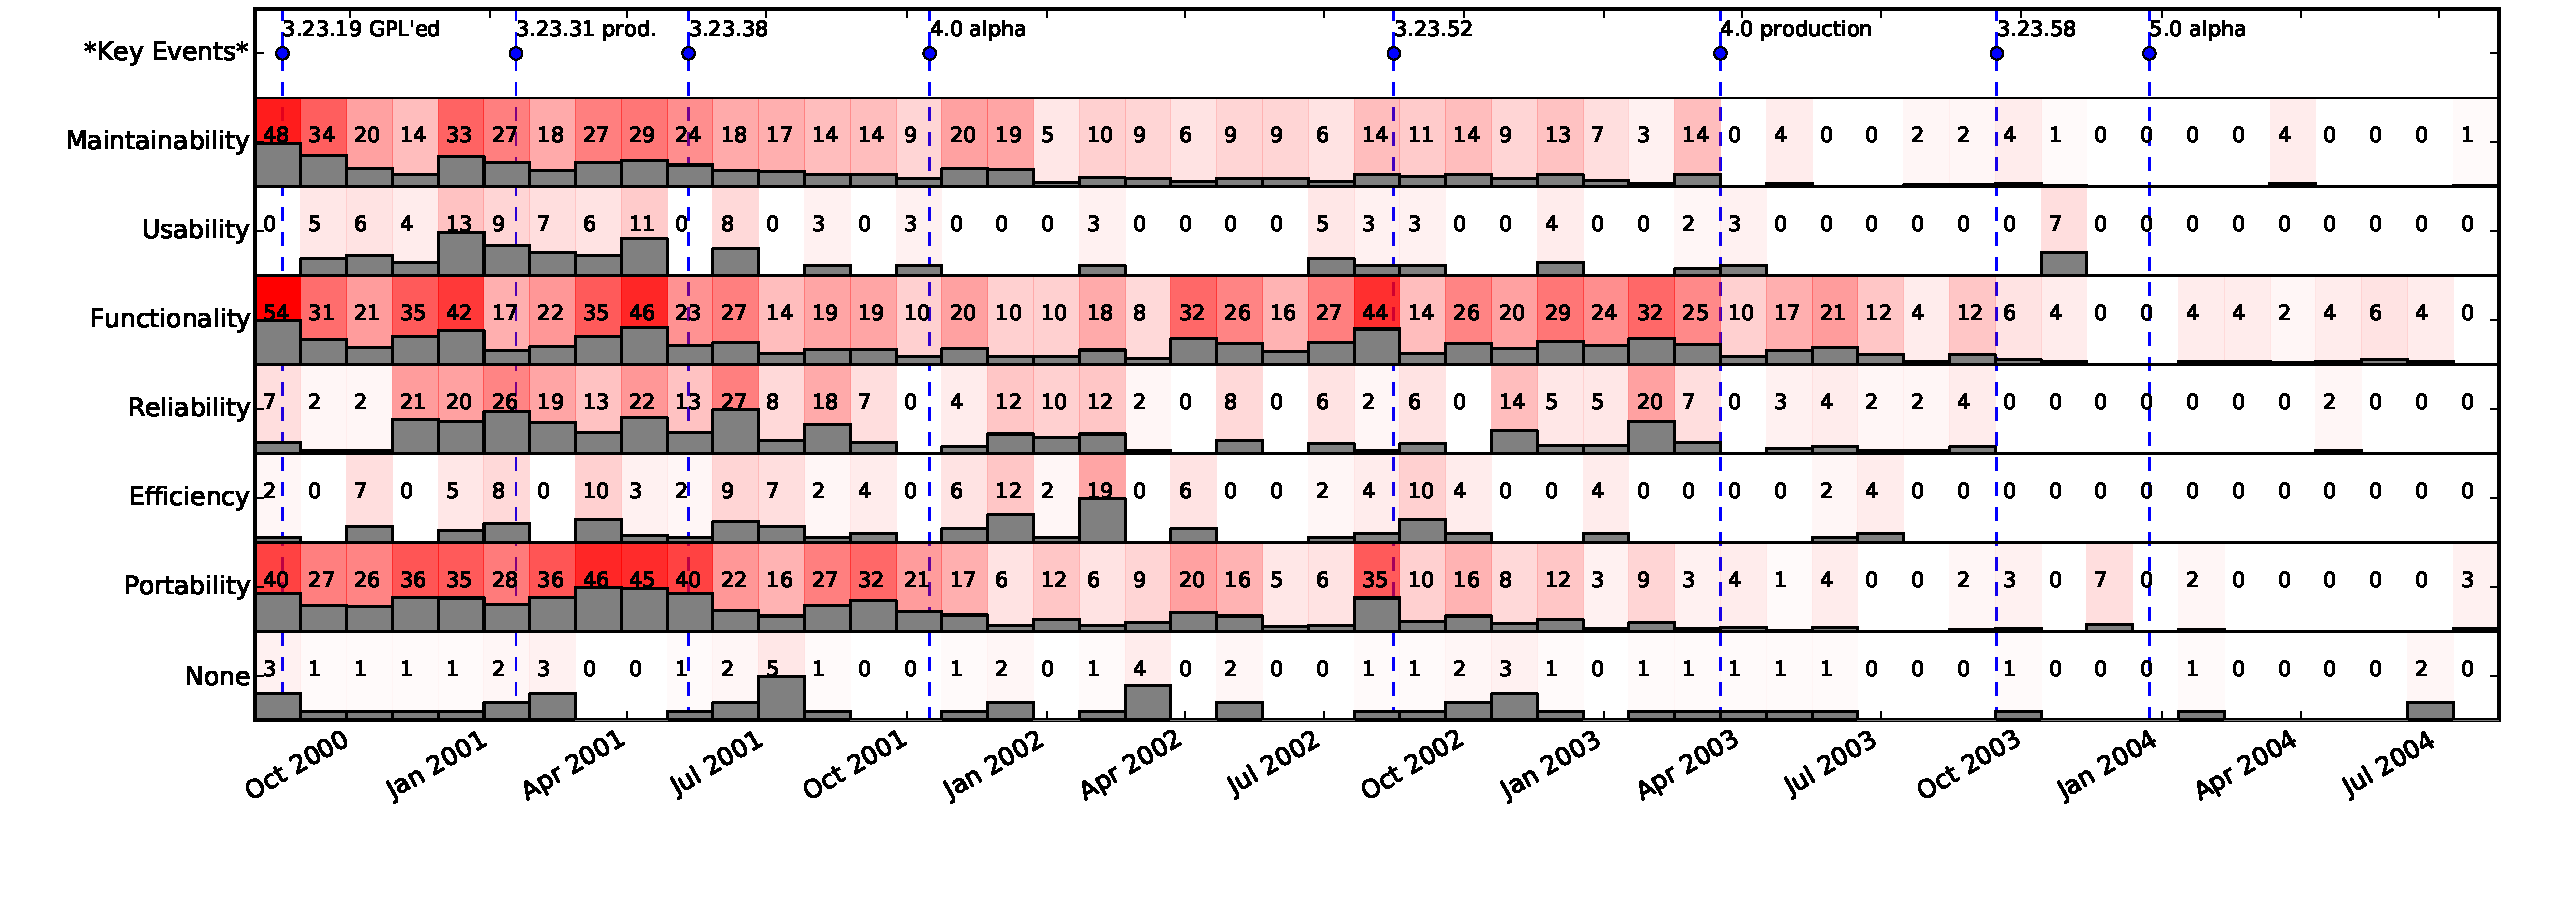
\includegraphics[width=\textwidth]{figures/mysql-timeline}
  \caption{MySQL 3.23: NFRs over time. Topic frequency relative to that quality is mapped to alpha (transparency) value.}
  \label{fig:mysql}
\end{figure*}

\section{NFRs between projects}

\subsection{Comparing MaxDB and MySQL}

\label{sec:comparison}
%\XXX{Not sure there's enough here to do that!}

We observed that MySQL had more topic subsets than MaxDB. MySQL 3.23 also had more topics and a longer recorded history than MaxDB 7.500. We tagged more MySQL topics with annotations than MaxDB topics yet both shared similarities. In terms of non-functional requirements both projects had long running trends that focused on functionality, maintainability, and portability, yet MaxDB had more of a focus on efficiency and reliability. MaxDB differed from MySQL since MaxDB was being actively developed, whereas halfway through our history of MySQL 3.23, other versions of MySQL were being actively developed: MySQL versions 4.0, 4.1, and eventually 5.0 and 5.1. In other words, MySQL 3.23 was being maintained rather than actively developed, whereas MaxDB 7.500 was being actively developed into MaxDB 7.6, and then maintained thereafter.

MySQL and MaxDB's machine learners did make decisions based off some shared words. Words that were used to classify topics that were shared between MySQL and MaxDB included: \textsf{bug, code, compiler, database, HP UX, delete, memory, missing, problems, removed, add, added, changed, problem, and test}. Adding these words to the word bags of \textsf{exp2} and \textsf{exp3} could improve performance while ensuring they were only domain specific.

With respect to the questions raised in section \ref{sec:suplearn}:

\textbf{Do label frequencies change over time?} -- Yes, MySQL's label
frequencies decreased as it got older. Usability and reliability
labels became more and more infrequent as it matured. Maintainability topics
became more prevalent as MaxDB matured.

\textbf{Do the different projects differ in their relative topic
  interest?} -- Yes. MySQL 3.23 had proportionally more
functionality labelled topics, while MaxDB had proportionally more
efficiency and portability related topics.
 

\begin{comment}
 shared-report.sh ; cat output/shared-j48-words 

      2 bug
      2 code
      2 compiler
      2 database
      2 Delete_
      2 HP_UX
      2 memory
      2 missing
      2 monty_mysql_com
      2 monty_mysql_fi
      2 problems
      2 Removed
      2 work__home_bk_mysql
      4 4_0
      4 Add
      4 added
      4 Changed
      4 problem
      6 Added
      6 test

\end{comment}


\subsection{Annotation observations}

We found many topics that were not non-functional requirements (NFRs) but were often related to them. For instance, concurrency was mentioned often in the commit logs and was related to correctness and reliability, because concurrency was troublesome. Configuration management and source control related changes appeared often and sometimes there were topics dedicated to configuration management. These kinds of changes are slightly related to maintainability. A non-functional change that was not quality-related was licensing and copyright; many changes were simply to do with updating copyrights or ensuring copyright or license headers were applied to files.

We noticed that occasionally the names of modules would conflict with words related to other non-functional requirements. For instance, optimizers are very common modules in database systems: both MySQL and MaxDB have optimizer modules. In MySQL the optimizer is mentioned but often the change deals with correctness or another quality. Despite this difference, the name of the module could fool our learners into believing the change was always about efficiency. Perhaps a project specific word-bag is needed in order to avoid automated mistakes due to the names of entities and modules of a software project.

\begin{comment}
A quick mind dump before I forget:
* portability was very popular
* there were many instances of concurrency
* There were often topics of crap commits with no comment
* might need more than the top words to compare
* Things like tests were noticable more by file type
* Configuration management is not part of the software quality ontology?
* I didn't tag none I tagged unknown, so that's some inconsistency between us
* There were a lot of copyright changes in mysql
* mysql had optimizer module which did not mean optimization
* I tried to assign reliability/bug for reliability bugs
  and Functionality/Correctness for fixes
* Some security changes came later
* Mysql 3.23 transitioned from a project being developed to
  a project being maintained, more frequent back-port bug-fixes
\end{comment}

\section{Limitations}
\subsection{Effectiveness}

%{Discuss how these are CHEAP techniques and although somewhat %inaccurate they don't require a tonne of work}

With ROC values ranging from $0.6$ to $0.8$ we can see there is promise in these attempts. \textsf{exp2} and \textsf{exp3} both indicate that static information can be used to help label topics without any training whatsoever. If the techniques used in \textsf{exp2} and \textsf{exp3} were combined with the supervised techniques we could probably reduce the training effort. 
Both Naive Bayesian learners and the word-list approaches were computationally efficient.  These results are promising, because the results are accurate enough to be useful, while still cheap enough to execute to be feasible as an automated or semi-automated method of labelling topics by their software qualities.


\subsection{Threats to validity}
\emph{Construct validity} issues include that we used only commit messages rather than mail or bug tracker messages. We also chose our taxonomy and the data to study. \emph{Internal validity} issues are to do with inter-rater reliability. \emph{External validity} issues are that our data originated from OSS database projects and thus might not be applicable to commercially developed software. Furthermore, our analysis techniques rely on a project's use of meaningful commit messages.


\section{Related work}

\begin{comment}
% Part of our effort with this project is to understand the qualitative and intentional aspects of requirements in software evolution, a notion we first discussed in \cite{ernst07icsm}. That idea is derived from, in part, work on narratives of software systems shown in academic work from Ant\'{o}n et al.~\cite{anton01}, or more general-purpose work from Waldo~\cite{waldo93}.

% Part of our effort with this project is to understand the qualitative and intentional aspects of requirements in software evolution, a notion we first discussed in \cite{ernst07icsm}. That idea is derived from, in part, work on narratives of software systems shown in academic work like \cite{anton01}, or more general-purpose works like \cite{waldo93}. 


% Not sure how do handle this
\end{comment}
The idea of extracting higher-level `concerns' (also known as `concepts', `aspects' or `requirements') has been approached in two ways. 

Cleland-Huang and her colleagues published work on mining requirements documents for non-functional requirements (NFR) (quality requirements)~\cite{Cleland-Huang2006}. One approach they tried was similar to this one, with keywords mined from NFR catalogues found in their previous work~\cite{chung99}. They managed recall of 80\% with precision of 57\% for the Security NFR, but could not find a reliable source of keywords for other NFRs. Instead, they developed a supervised classifier by using human experts to identify an NFR training set. There are several reasons we did not follow this route. One, we believe we have a more comprehensive set of terms due to the taxonomy we chose. Secondly, we wanted to compare across projects. Their technique was not compared across different projects and the applicability of the training set to different corpora is unclear. A common taxonomy allows us to make inter-project comparison (subject to the assumption that all projects conceive of these terms in the same way). Thirdly, while the objective of Cleland-Huang's study was to identify new NFRs (for system development) our study assumes these NFRs are latent in the textual documents of the project. Finally, the source text we use is less structured than their requirements documents.

In the same vein, Mockus and Votta~\cite{Mockus00} studied a large-scale industrial change-tracking system. They also leveraged WordNet, but only for word roots. They felt the synonyms would be non-specific and cause errors. A nice contribution was access to system developers, with whom they could validate their labels. Since we try to bridge different organizations, these interviews are infeasible (particularly in the distributed world of open-source software).

The other approach is to start with code repositories, and try to extract concerns from there. Marcus et al.~\cite{marcus04wcre} describe their use of Latent Semantic Indexing to identify commonly occurring concerns for software maintenance. Some results were interesting, but their precision was quite low. ConcernLines~\cite{treude09cl} shows tag occurrence using colour intensity. They mined change request tags (such as `milestone 3') and used these to make evolutionary analyses of a single product. The presence of a well-maintained set of tags is obviously essential to the success of this technique.

\begin{comment}
%We maintain that these results require more substantive manipulation before being reported to, for example, management. Like any large-scale data analysis project, it requires skill to derive the implications. Hooking the backend results directly to a reporting tool is unlikely to produce useful results.

% There has been an explosion of interest in mining OSS repositories. Godfrey and Tu \cite{godfrey00} were among the first to use this data to assess software evolution. They discussed how well the growth of Linux was predicted by laws that Lehman and colleagues \cite{lehman85} proposed. More recently, Herraiz et al. \cite{herraiz07icsm} predicted OSS growth using time series analysis. Like us, they refer to release windows as a useful unit of analysis. 
\end{comment}


Mens et al.~\cite{mens08icsm} conducted an empirical study of Eclipse, the open source software (OSS) source code editor, to verify the claims of Lehman~\cite{lehman97sms}. They concerned themselves with source code only, and found Law Seven, ``Declining Quality'', to be too difficult to assess: ``[we lacked an] appropriate measurement of the evolving quality of the system as perceived by the users \cite[p. 388]{mens08icsm}''. This paper examines the notions of quality in terms of a consistent ontology, as Mens et al. call for in their conclusions.

Mei et al.~\cite{Mei2007} use context information to automatically name topics. They describe probabilistic labelling, using the frequency distribution of words in a topic to create a meaningful phrase. They do not use external domain-specific information as we do.
In \cite{ernst10refsq}, we describe our earlier project, similar to this, to identify change in quality requirements in GNOME software projects; our approach is solely text-matching, however, it does not leverage machine learning strategies.

\begin{comment}
% comment out or not
% Massey~\cite{massey02icse} and Scacchi~\cite{scacchi02,scacchi05b} looked at the topic of requirements in open-source software. Their work discusses the source of the requirements and how they are used in the development process. German~\cite{german03gnome} looked at GNOME specifically, and listed several sources for requirements: leader interest, mimicry, brainstorming, and prototypes. None of this work  addressed quality requirements in OSS, nor did it examine requirements trends.

% Hindle et al. \cite{Hindle2007} examined release patterns in OSS. They showed that there is a difference between projects regarding maintenance techniques. This supports our result that software qualities are not discussed with the same frequency across projects.
\end{comment}

\section{Conclusions and future work}

We demonstrated that static but domain-specific knowledge can improve unsupervised labelling of extracted topics. Our \textsf{exp2} experiment used small accurate word bags to label topics but performed just as well as \textsf{exp3}, which used many more general terms from WordNet. We then showed that with some supervision, and by using efficient machine learners based on Naive Bayesian classifiers, we could improve the accuracy of automatic labelling topics even further.

Our manual inspection and annotation of the topics extracted from MySQL and MaxDB revealed that many of the extracted topics dealt with non-functional requirements, and these topics were spread across the entire history of a project. In the cases of MaxDB and MySQL, portability was a constant maintenance concern and was prevalent throughout the entire lifetime of the projects.

We showed that non-functional requirements are often trending topics, that non-functional requirements are quite common in developer topics, and that there are efficient methods of semi-automating and automating topic labelling.

There are several avenues of further investigation.  We want to investigate developer attitudes related to these labels: i.e., when we label a topic, was the developer expressing positive or negative qualities about that label?  It is difficult to map abstract qualities to particular messages. Is a ``quality'' discussion about more than just corrective maintenance? %In this study we take the position that any type of maintenance has to do with software quality.

%XXX can save space here!
\section{Appendix}
Our data and scripts are available at \url{http://softwareprocess.es/nomen/}

\bibliographystyle{abbrv}
%\bibliographystyle{IEEEtran}
\bibliography{icpc}

\end{document}

